% !TEX root = ../thesis.tex
%
\chapter{External Non-local Self-Similarity Prior for Additive White Gaussian Noise}
\label{sec:external}

%\cleanchapterquote{Innovation distinguishes between a leader and a follower.}{Steve Jobs}{(CEO Apple Inc.)}

\section{Introduction}
\begin{figure}
\centering
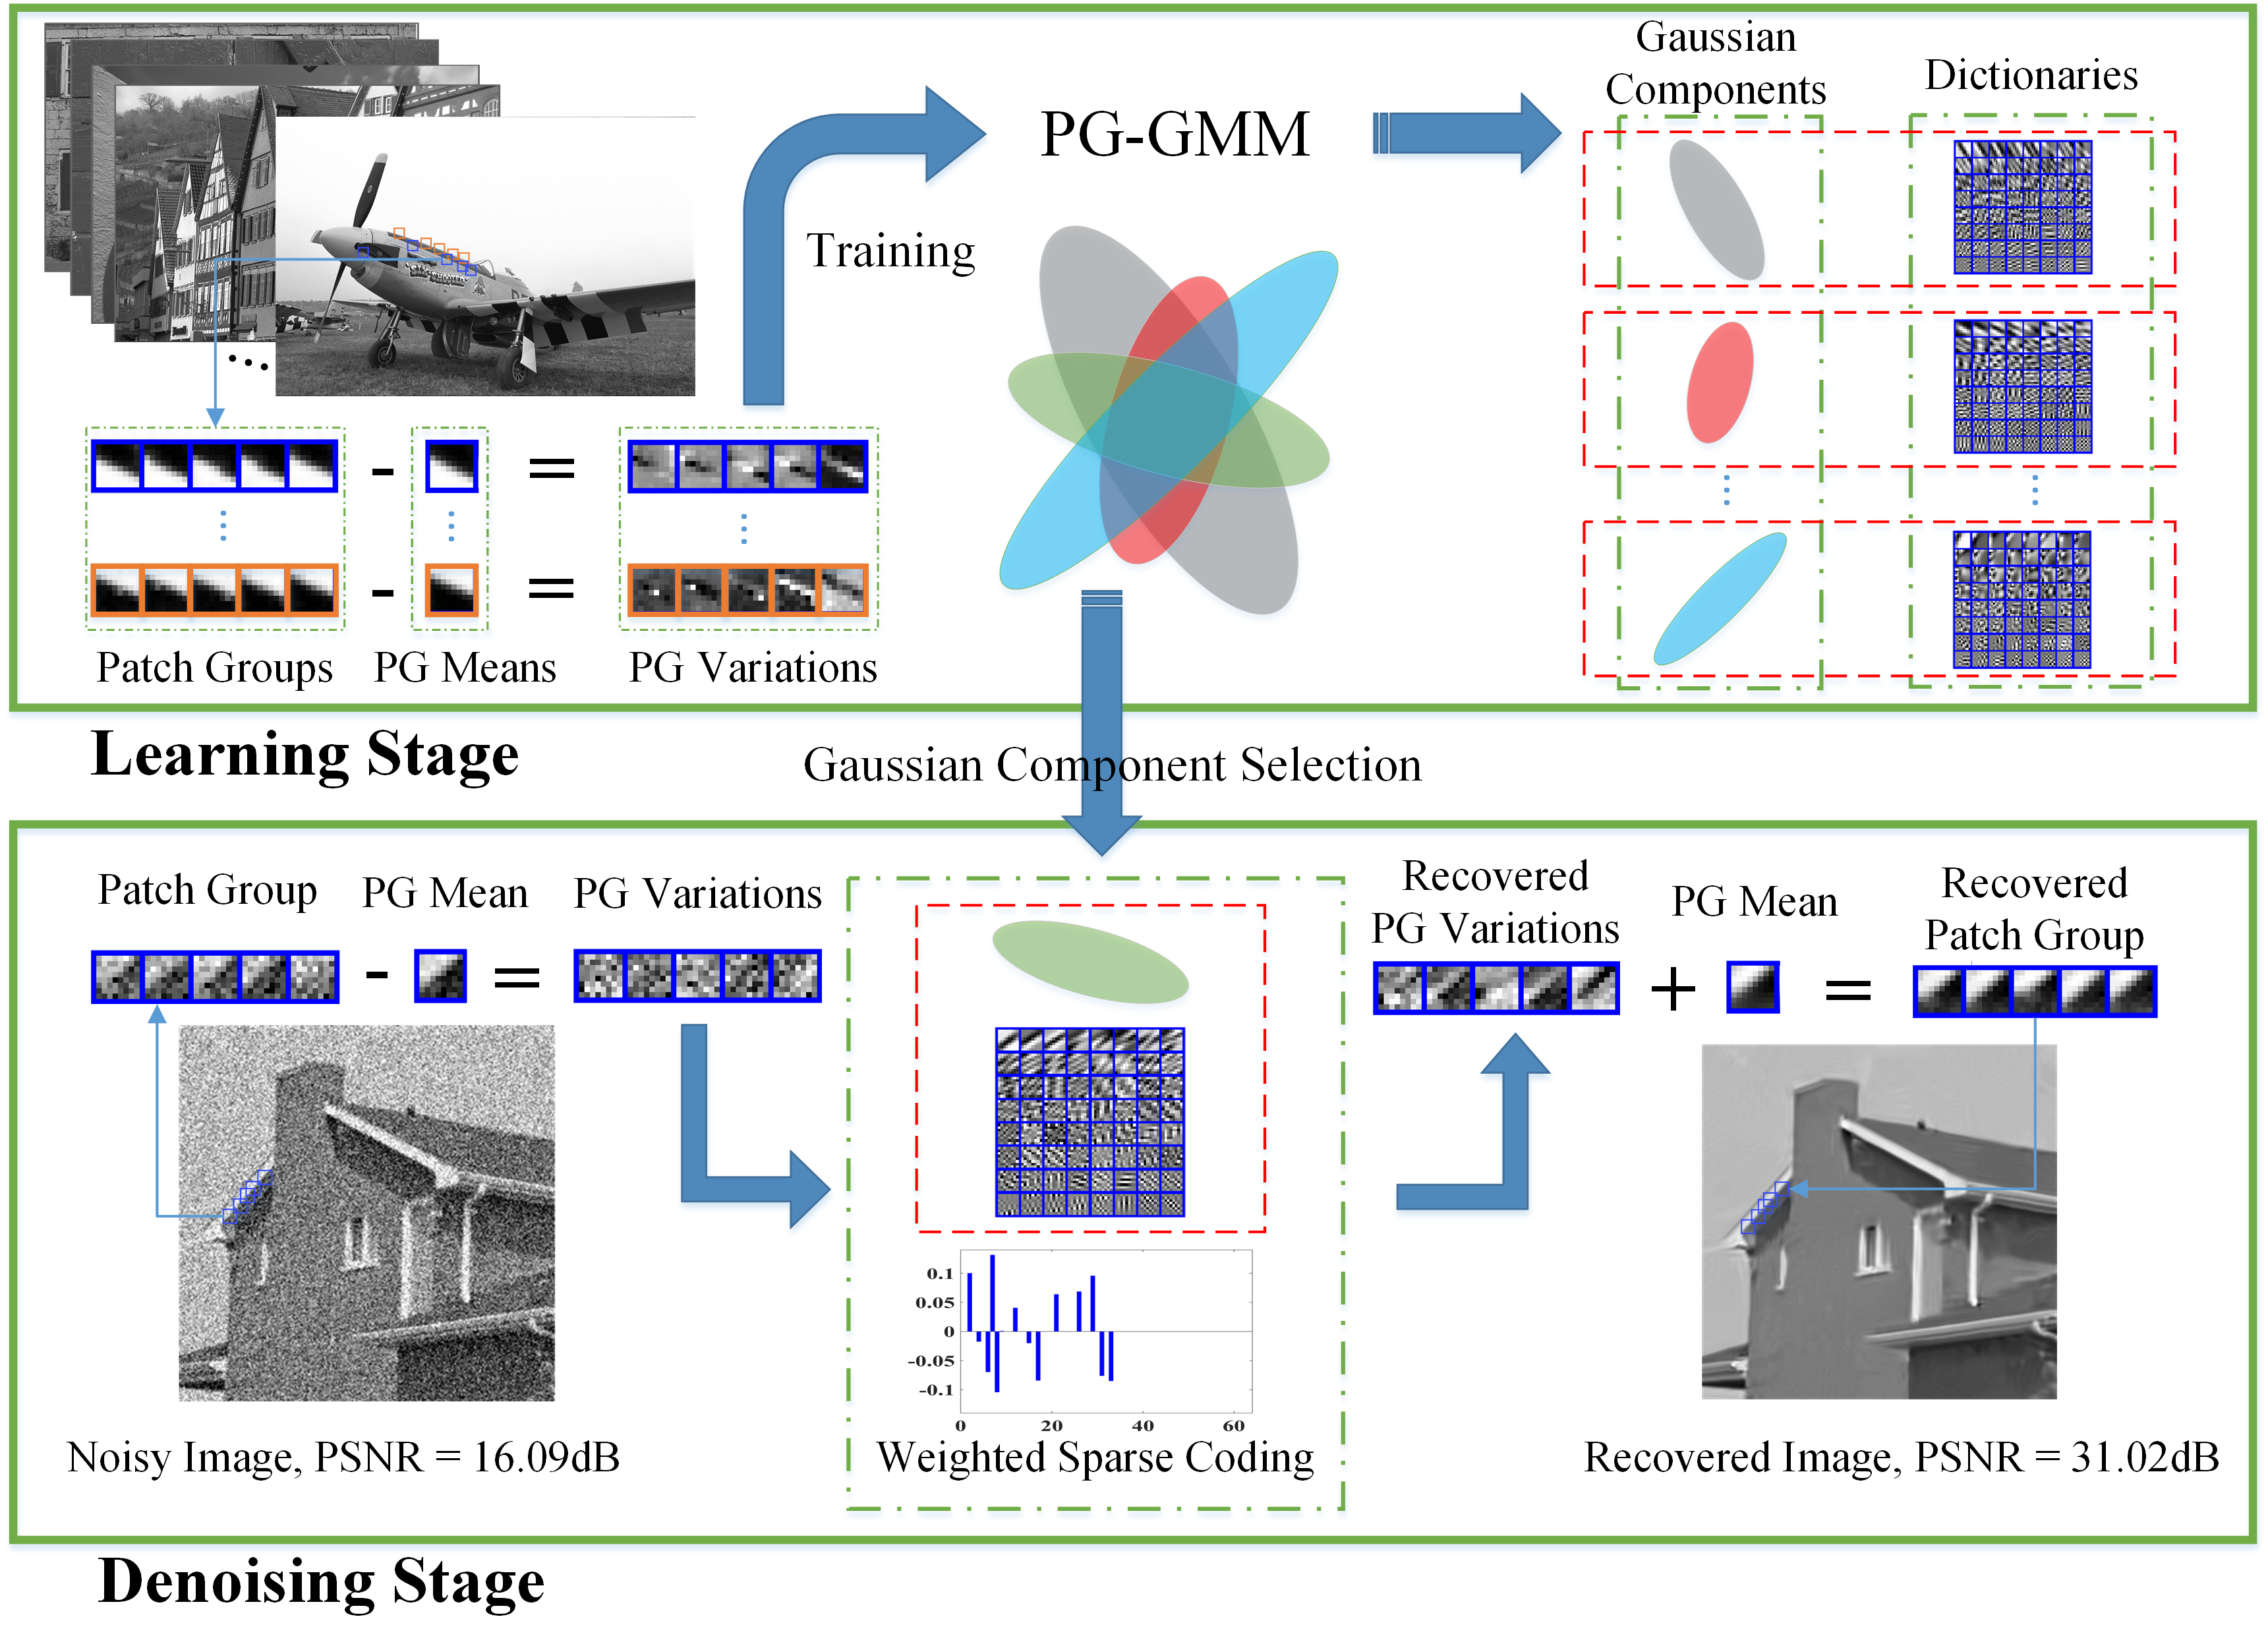
\includegraphics[width=0.74\linewidth]{images/pgpd/flowchart2.png}
\caption{Flowchart of the proposed patch group based prior learning and image denoising framework.}
\label{fig1}
\end{figure}

As a classical problem in low level vision, image denoising has been extensively studied, yet it is still an active topic for that it provides an ideal test bed for image modeling techniques. In general, image denoising aims to recover the clean image $\bm{x}$ from its noisy observation $\bm{y} = \bm{x} + \bm{v}$, where $\bm{v}$ is assumed to be additive white Gaussian noise.\ A variety of image denoising methods have been developed in past decades, including filtering based methods \cite{Tomasi1998}, diffusion based methods \cite{PeronaMalik1990}, total variation based methods \cite{rudin1992nonlinear,osher2005iterative}, wavelet/curvelet based methods \cite{softthresholding,bayesshrink,curvelet}, sparse representation based methods \cite{ksvd,lssc,ncsr}, nonlocal self-similarity based methods \cite{nlm,bm3d,nnm,wnnm}, etc.

Image modeling plays a central role in image denoising. By modeling the wavelet transform coefficients as Laplacian distributions, many wavelet shrinkage based denoising methods such as the classical soft-thresholding \cite{softthresholding} have been proposed.\ Chang et al. modeled the wavelet transform coefficients as generalized Gaussian distribution, and proposed the BayesShrink \cite{bayesshrink} algorithm.\ By considering the correlation of wavelet coefficients across scales, Portilla et al.  \cite{blsgsm} proposed to use Gaussian Scale Mixtures for image modeling and achieved promising denoising performance. It is widely accepted that natural image gradients exhibit heavy-tailed distributions \cite{weiss}, and the total variation (TV) based methods \cite{rudin1992nonlinear,osher2005iterative} actually assume Laplacian distributions of image gradients for denoising. The Fields of Experts (FoE) \cite{foe} proposed by Roth and Black models the filtering responses with Student's t-distribution to learn filters through Markov Random Field (MRF) \cite{Bishop}. Recently, Schmidt and Roth proposed the cascade of shrinkage fields (CSF) to perform denoising efficiently \cite{csf}.

Instead of modeling the image statistics in some transformed domain (e.g., gradient domain, wavelet domain or filtering response domain), another popular approach is to model the image priors on patches. One representative is the sparse representation based scheme which encodes an image patch as a linear combination of a few atoms selected from a dictionary \cite{olshausen1996emergence,olshausen1997sparse,ksvd}. The dictionary can be chosen from the off-the-shelf dictionaries (e.g., wavelets and curvelets), or it can be learned from natural image patches.\ The seminal work of K-SVD \cite{ksvdtsp,ksvd} has demonstrated promising denoising performance by dictionary learning, which has yet been extended and successfully used in various image processing and computer vision applications \cite{srcolor,srcvpr,lcksvd}. By viewing image patches as samples of a multivariate variable vector and considering that natural images are non-Gaussian, Zoran and Weiss \cite{epll,gmmnips} and Yu et al.  \cite{ple} used Gaussian Mixture Model (GMM) to model image patches, and achieved state-of-the-art denoising and image restoration results, respectively.

Natural images often have many repetitive local patterns, and a local patch can have many similar patches to it across the whole image.\ The so-called nonlocal self-similarity (NSS) prior is among the most successful priors for image restoration.\ The nonlocal means \cite{nlm} and nonlocal regularization \cite{nlr} methods improve much the image denoising performance over the conventional local self-similarity based methods. Dabov et al. \cite{bm3d} constructed 3D cubes of nonlocal similar patches and conducted collaborative filtering in the sparse 3D transform domain.\ The so-called BM3D algorithm has become a benchmark in image denoising. Mairal et al. \cite{lssc} proposed the LSSC algorithm to exploit NSS via group sparse coding.\ The NSP \cite{nsp} method fits the singular values of NSS patch matrix by Laplacian distribution.\ Dong et al. \cite{ncsr} unified NSS and local sparse coding into the so-called NCSR framework, which shows powerful image restoration capability. By assuming that the matrix of nonlocal similar patches has a low rank structure, the low-rank minimization based methods \cite{nnm,wnnm} have also achieved very competitive denoising results. 

Though NSS has demonstrated its great success in image denoising, in most existing methods only the NSS of noisy input image is used for denoising.\ For example, in BM3D \cite{bm3d} the nonlocal similar patches of a noisy image are collected as a cube for collaborative filtering. In NCSR \cite{ncsr}, the nonlocal means are subtracted in the sparse domain to regularize the sparse coding of noisy patches. In WNNM \cite{wnnm}, the low-rank regularization is enforced to recover the latent structure of the matrix of noisy patches. We argue that, however, such utilizations of NSS are not effective enough because they neglect the NSS of clean natural images, which can be pre-learned for use in the denoising stage. \ To the best of our knowledge, unfortunately, so far there is not an explicit NSS prior model learned from natural images for image restoration. 

With the above considerations, in this work we propose to learn explicit NSS models from natural images, and apply the learned prior models to noisy images for high performance denoising. The flowchart of the proposed method is illustrated in Fig.\ \ref{fig1}.\ In the learning stage, we extract millions of patch groups (PG) from a set of clean natural images.\ A PG is formed by grouping the similar patches to a local patch in a large enough neighborhood.\ A PG based GMM (PG-GMM) learning algorithm is developed to learn the NSS prior for the PGs. In the denoising stage, the learned PG-GMM will provide dictionaries as well as regularization parameters, and a simple weighted sparse coding model is developed for image denoising.\ Our extensive experiments validated that the proposed PG prior based denoising method outperforms many state-of-the-art algorithms quantitatively (in PSNR) while being much more efficient. More importantly, it delivers the best qualitative denoising results with finer details and less artifacts, owe to the NSS prior learned from clean natural images.   

%-------------------------------------------------------------------------
\section{Patch Group Based Prior Modeling of Nonlocal Self-Similarity}
Image nonlocal self-similarity (NSS) has been widely adopted in patch based image denoising and other image restoration tasks \cite{nlm,bm3d,lssc,ncsr,wnnm}.\ Despite the great success of NSS in image restoration, most of the existing works exploit the NSS only from the degraded image.\ Usually, for a given patch in the degraded image, its nonlocal similar patches are collected, and then the nonlocal means \cite{nlm}, or 3D transforms \cite{bm3d}, or some regularization terms \cite{lssc,ncsr,wnnm,srcolor} can be introduced for image restoration. However, how to learn the NSS prior from clean natural images and apply it to image restoration is still an open problem. In this work, we make the first attempt on this problem, and develop a patch group (PG) based NSS prior learning scheme.  
\subsection{Patch Group and Group Mean Subtraction}
For each local patch (size: $p\times p$) of a given clean image, we can find the first $M$ most similar nonlocal patches to it across the whole image. In practice, this can be done by Euclidean distance based block matching in a large enough local window of size $W\times W$. A PG is formed by grouping the $M$ similar patches, denoted by $\{\bm{x}_{m}\}_{m=1}^{M}$, where $\bm{x}_{m}\in \mathbb{R}^{p^{2}\times1}$ is a patch vector. The mean vector of this PG is $\bm{\mu}=\frac{1}{M}\sum_{m=1}^{M}\bm{x}_{m}$, and $\bm{\overline{x}}_{m}=\bm{x}_{m}-\bm{\mu}$ is the group mean subtracted patch vector. We call
\begin{equation}
\label{equ1}
\overline{\bm{X}}\triangleq \{\overline{\bm{x}}_{m}\}, m=1,...,M
\end{equation}
the group mean subtracted PG, and it will be used to learn the NSS prior in our work. 

In Fig.\ \ref{fig2}, we show two different PGs, their group means, and the PGs after mean subtraction.\ One can see that before mean subtraction, the two PGs have very different local structures.\ After mean subtraction, the two PGs will have very similar variations.\ This greatly facilitates the prior learning because the possible number of patterns is reduced, while the training samples of each pattern are increased. We will discuss further the benefits of mean subtraction and the associated prior model learning in Section 2.4.   
\subsection{PG-GMM Learning}
From a given set of natural images, we can extract $N$ PGs, and we denote one PG as
\begin{equation}
\label{equ2}
\overline{\bm{X}}_{n}\triangleq \{\overline{\bm{x}}_{n,m}\}_{m=1}^{M}, n=1,...,N.
\end{equation}
The PGs $\{\bm{\overline{X}}_{n}\}$ contain a rich amount of NSS information of natural images, and the problem turns to how to learn explicit prior models from $\{\bm{\overline{X}}_{n}\}$. Considering that Gaussian Mixture Model (GMM) has been successfully used to model the image patch priors in EPLL \cite{epll} and PLE \cite{ple}, we propose to extend patch based GMM to patch group based GMM (PG-GMM) for NSS prior learning.
\begin{figure}
\centering
\centering
\includegraphics[width=0.7\linewidth]{images/pgpd/2pgs.png}
\caption{Different patch groups (PG) share similar PG variations.}
\label{fig2}
\end{figure}

With PG-GMM, we aim to learn a set of $K$ Gaussians $\{\mathcal{N}(\bm{\mu}_{k},\bm{\Sigma}_{k})\}$ from $N$ training PGs $\{\bm{\overline{X}}_{n}\}$, while requiring that all the $M$ patches $\{\bm{\overline{x}}_{n,m}\}$  in PG $\bm{\overline{X}}_{n}$ belong to the same Gaussian component and assume that the patches in the PG are independently sampled. Note that such an assumption is commonly used in patch based image modeling \cite{ksvd,lssc}. Then, the likelihood of $\{\bm{\overline{X}}_{n}\}$ can be calculated as
\begin{equation}
\label{equ3}
P(\bm{\overline{X}}_{n})  = \sum\nolimits_{k=1}^{K}\pi_{k}\prod\nolimits_{m=1}^{M}\mathcal{N}(\bm{\overline{x}}_{n,m}|\bm{\mu}_{k},\bm{\Sigma}_{k}).
\end{equation}
By assuming that all the PGs are independently sampled, the overall objective likelihood function is $\mathcal{L} = \prod_{n=1}^{N}P(\bm{\overline{X}}_{n})$. Taking the log of it, we maximize the following objective function for PG-GMM learning
\begin{equation}
\label{equ4}
\begin{split}
\ln\mathcal{L}=\sum_{n=1}^{N} \ln(\sum_{k=1}^{K}\pi_{k}\prod_{m=1}^{M}\mathcal{N}(\bm{\overline{x}}_{n,m}|\bm{\mu}_{k},\bm{\Sigma}_{k})).
\end{split}
\end{equation}

As in GMM learning \cite{Bishop}, we introduce hidden variables $\{\Delta_{nk}|n=1,...,N;k=1,...,K\}$ to optimize (\ref{equ4}). If PG $\bm{\overline{X}}_{n}$ belongs to the $k$th component, $\Delta_{nk}=1$; and $\Delta_{nk}=0$ otherwise. Then the EM algorithm \cite{em} can be used to optimize (\ref{equ4}) via two alternative steps. In the E-Step, by the Bayes' formula, the expected value of $\Delta_{nk}$ is
\begin{equation}\label{equ5}
\gamma_{nk}=\frac{\pi_{k}\prod_{m=1}^{M}\mathcal{N}(\bm{\overline{x}}_{n,m}|\bm{\mu}_{k},\bm{\Sigma}_{k})}{\sum_{l=1}^{K}\pi_{l}\prod_{m=1}^{M}\mathcal{N}(\bm{\overline{x}}_{n,m}|\bm{\mu}_{l},\bm{\Sigma}_{l})}.
\end{equation}
In the M-step, since for each PG $\bm{\overline{X}}_{n}$, $\sum_{m=1}^{M}\bm{\overline{x}}_{n,m}=\bm{0}$, we have
\begin{equation}
\label{equ6}
\bm{\mu}_{k} = \frac{\sum_{n=1}^{N}\gamma_{nk}\sum_{m=1}^{M}\bm{\overline{x}}_{n,m}}{\sum_{n=1}^{N}\gamma_{nk}}=\bm{0},
\end{equation}
\begin{equation}\label{equ7}
\bm{\Sigma}_{k} = \frac{\sum_{n=1}^{N}\gamma_{nk}\sum_{m=1}^{M}\bm{\overline{x}}_{n,m}\bm{\overline{x}}_{n,m}^{T}}{\sum_{n=1}^{N}\gamma_{nk}}.
\end{equation}
The calculations of $\pi_{k}=\frac{1}{N}\sum_{n=1}^{N}\gamma_{nk}$ are similar to \cite{Bishop}.

By alternating between the E-step and the M-step, the model parameters will be updated iteratively, and the update in each iteration can guarantee to increase the value of the log-likelihood function (\ref{equ5}), and the EM algorithm will converge \cite{Bishop,emconvergence}. Fig. \ref{fig3} shows the convergence curve of the proposed PG-GMM algorithm by using the Kodak PhotoCD Dataset (\url{http://r0k.us/graphics/kodak/}) for training.
\begin{figure}[t]
\centering
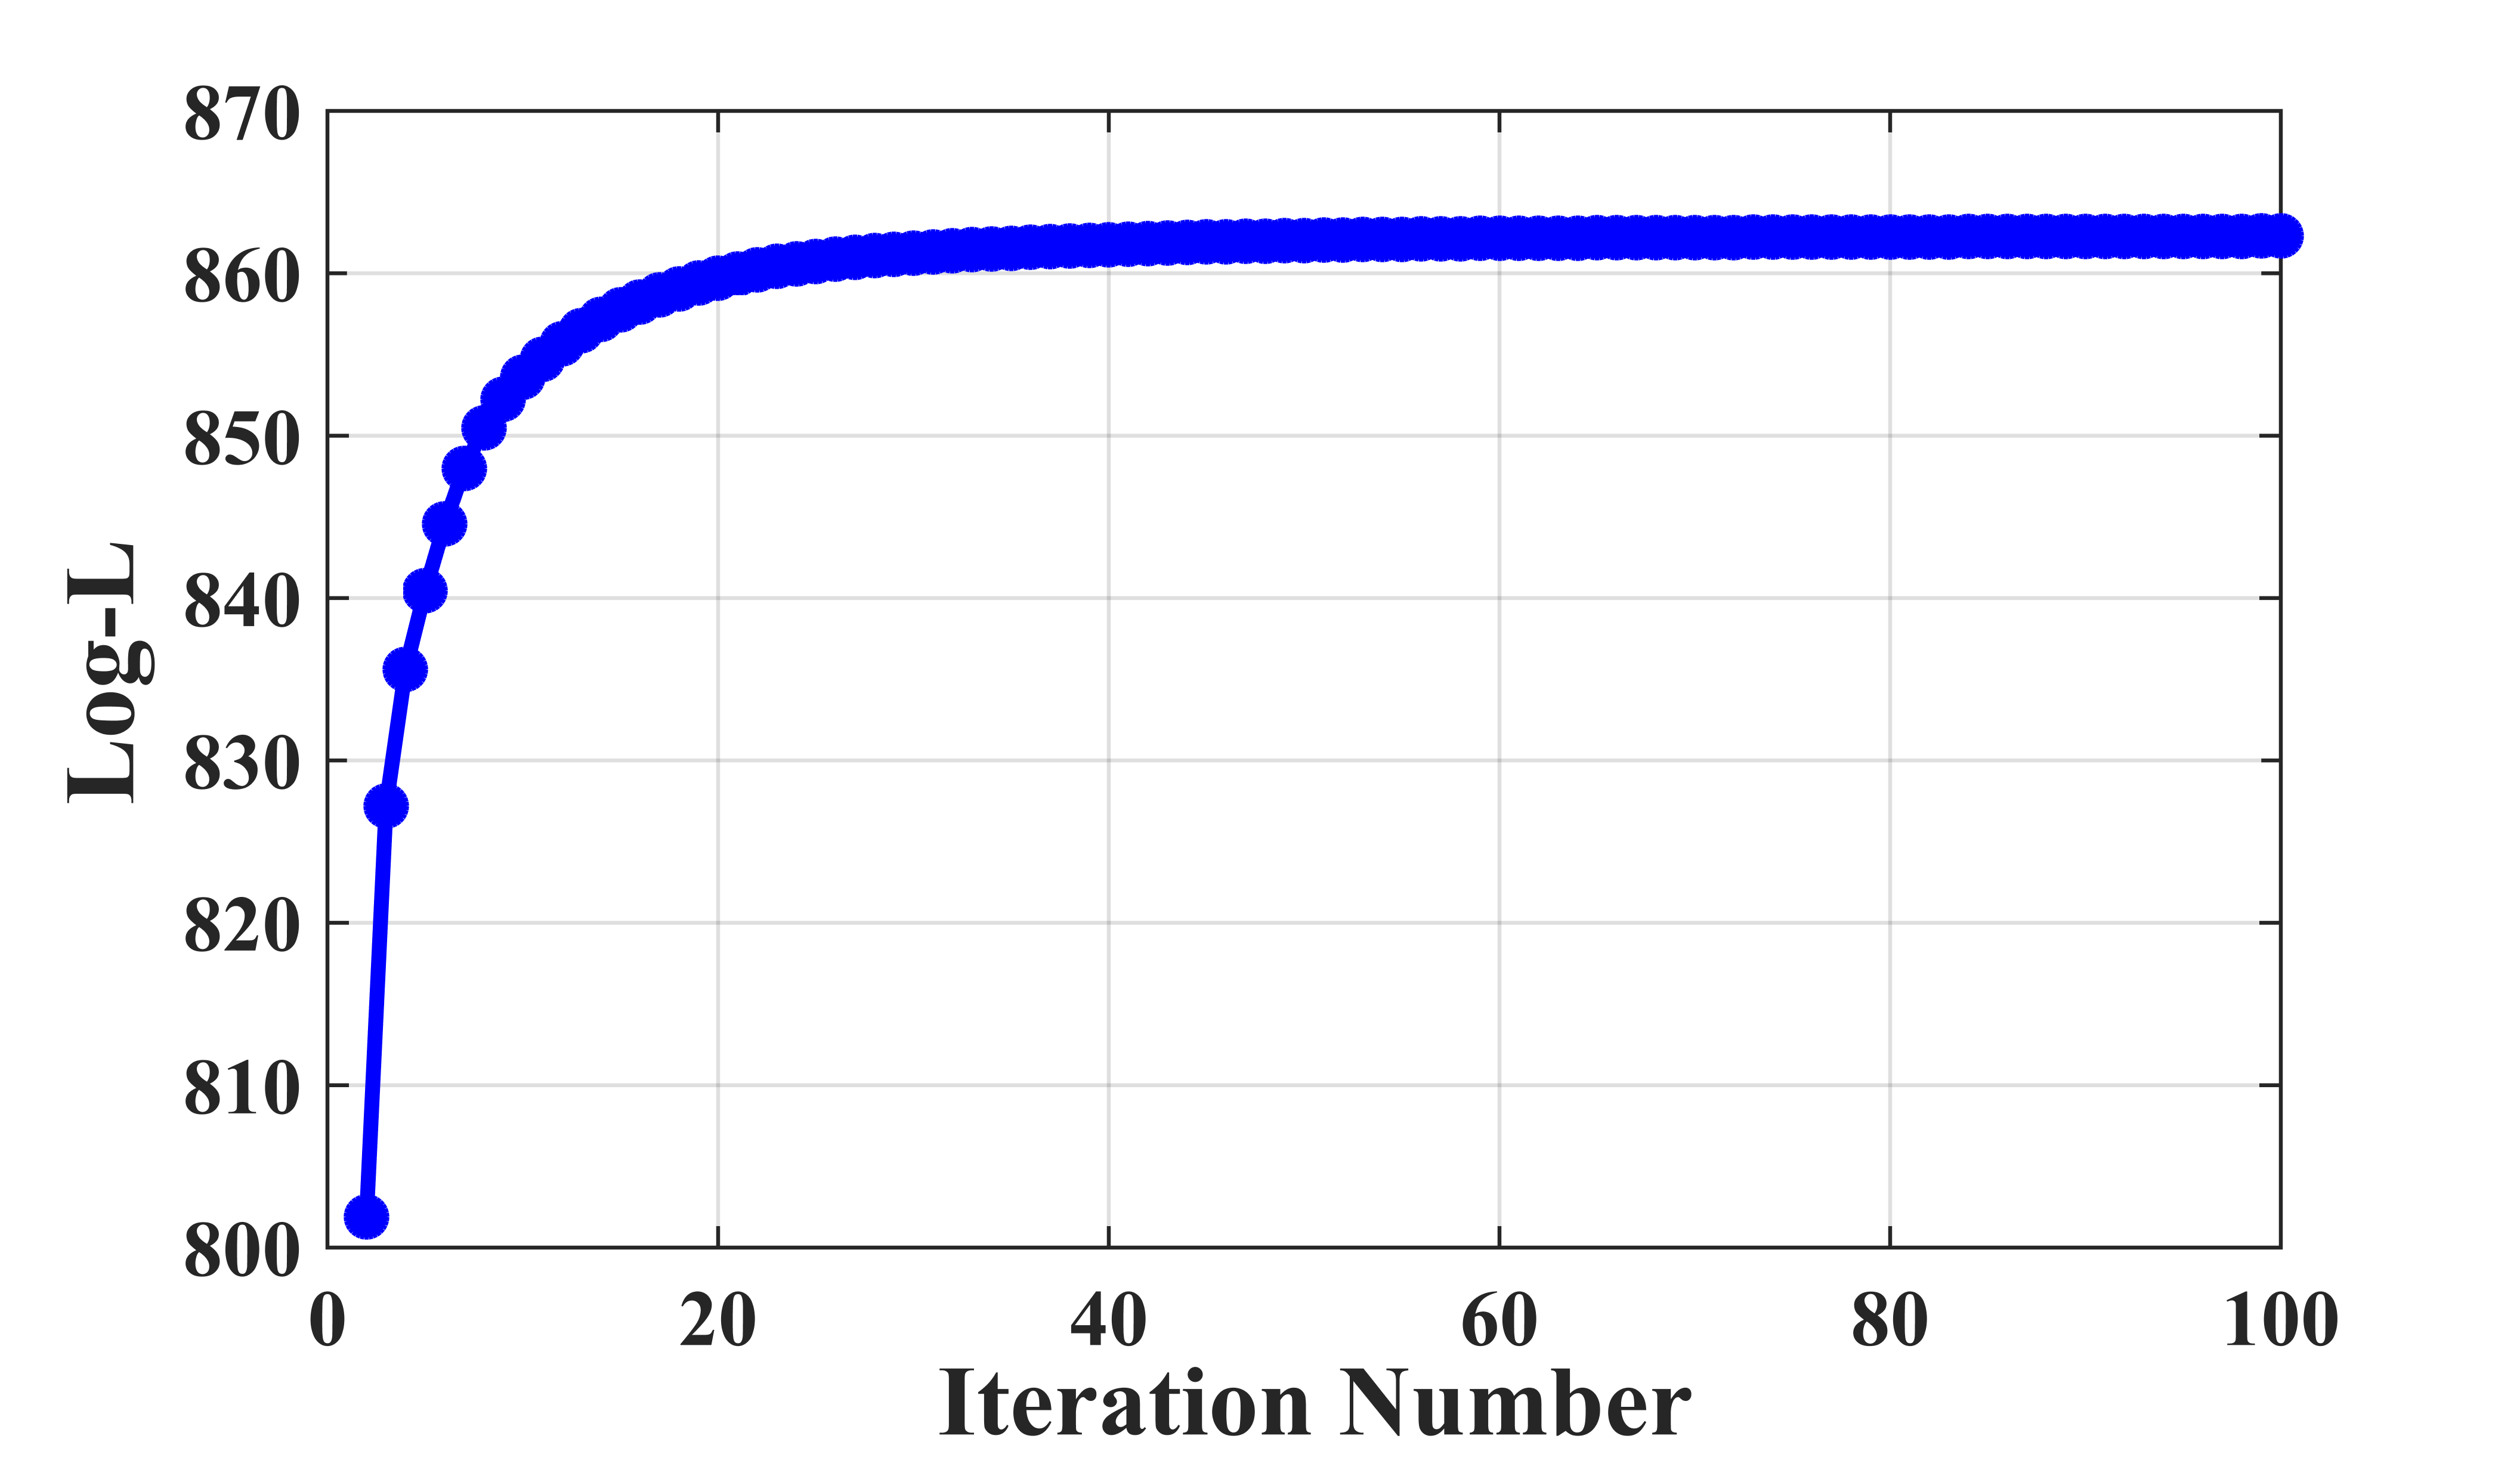
\includegraphics[width=0.75\linewidth]{images/pgpd/cvgc.png}
\caption{The convergence curve of log-likelihood in PG-GMM training on the Kodak PhotoCD Dataset.
}
\label{fig3}
\end{figure}

\subsection{Complexity Analysis}
In the training stage, there are $N$ PGs, each of which has $M$ patches, and hence we have $N\times M$ patches. In the M-step, we only need to calculate the covariance matrices since the mean of each Gaussian component is zero. The cost of this step is $O(p^{4}MN)$. In the E-step, the cost is $O(p^{6}MN)$. Suppose that the number of iterations is $T$, the overall complexity of PG-GMM training is $O(p^{6}MNT)$.
\subsection{Discussions}
GMM has been used for patch based image prior learning and achieved promising results, e.g., EPLL \cite{epll} and PLE \cite{ple}. In this paper, we extend the patch based image prior learning to PG based prior learning to model the NSS information.\ The developed PG-GMM method has some important advantages over the patch based GMM method.

First, in patch based GMM, the mean value of each patch is subtracted before learning the Gaussian components. This is to remove the DC (direct current) of each patch but will not change the essential structure of a patch. However, in PG-GMM the mean vector of all patches in a group is calculated and subtracted from each patch, and hence the structure of each patch is changed. As a result, many patches which originally have different local patterns may become similar after group mean subtraction (please refer to Fig. \ref{fig2} for an example). This makes the PG-GMM learning process easier and more stable. 

Second, as can be seen in Eq.\ (\ref{equ9}), the mean vector of each Gaussian component in PG-GMM is naturally a zero vector.\ This implies that we only need to learn the covariance matrix of each component without considering its mean. However, in patch based GMM \cite{epll}, the mean vectors of Gaussians can only be forced to zero and there is no theoretical guarantee for this.

Third, due to reduction of possible patterns in PG-GMM and the reduced number of variables to learn, we do not need to set a large number of Gaussian components in PG-GMM learning. For example, in EPLL \cite{epll}, 200 Gaussian components are learned to achieve competing denoising performance with BM3D \cite{bm3d}, while in PG-GMM learning only 32 Gaussian components are enough to outperform BM3D (please refer to the experimental section for details).
%-------------------------------------------------------------------------
\section{Image Denoising by Patch Group Priors}
\subsection{Denoising Model}
Given a noisy image $\bm{y}$, like in the PG-GMM learning stage, for each local patch we search for its similar patches in a window centered on it to form a PG, denoted by $\bm{Y} = \{\bm{y}_{1},...,\bm{y}_{M}\}$. Then the group mean of $\bm{Y}$, denoted by $\bm{\mu}_{y}$, is calculated and subtracted from each patch, leading to the mean subtracted PG $\bm{\overline{Y}}$. We can write $\bm{\overline{Y}}$ as $\bm{\overline{Y}}=\bm{\overline{X}}+\bm{V}$, where $\bm{\overline{X}}$ is the corresponding clean PG and $\bm{V}$ contains the corrupted noise. The problem then turns to how to recover $\bm{\overline{X}}$ from $\bm{\overline{Y}}$ by using the learned PG-GMM priors. Note that the mean $\bm{\mu}_{y}$ of $\bm{\overline{Y}}$  is very close to the mean of $\bm{\overline{X}}$ since the mean vector of noise $\bm{V}$ is nearly zero.\ $\bm{\mu}_{y}$ will be added back to the denoised PG to obtain the denoised image. 

\subsubsection{Gaussian Component Selection}
For each $\bm{\overline{Y}}$, we select the most suitable Gaussian component to it from the trained PG-GMM. As in \cite{epll}, suppose that the variance of Gaussian white noise corrupted in the image is $\sigma^{2}$, the covariance matrix of the $k$th component will become $\bm{\Sigma}_{k}+\sigma^{2}\bm{I}$, where $\bm{I}$ is the identity matrix. The selection can be done by checking the posterior probability that $\bm{\overline{Y}}$ belongs to the $k$th Gaussian component:
\begin{equation}\label{equ8}
P(k|\bm{\overline{Y}})=\frac{\prod_{m=1}^{M}\mathcal{N}(\bm{\overline{y}}_{m}|\bm{0},\bm{\Sigma}_{k}+\sigma^{2}\bm{I})}{\sum_{l=1}^{K}\prod_{m=1}^{M}\mathcal{N}(\bm{\overline{y}}_{m}|\bm{0},\bm{\Sigma}_{l}+\sigma^{2}\bm{I})}.
\end{equation}
Taking log-likelihood of (\ref{equ8}), we have
\begin{equation}\label{equ9}
\setlength{\abovedisplayskip}{3pt}
\setlength{\belowdisplayskip}{3pt}
\ln P(k|\bm{\overline{Y}}) = \sum\nolimits_{m=1}^{M}\ln\mathcal{N}(\bm{\overline{y}}_{m}|\bm{0},\bm{\Sigma}_{k}+\sigma^{2})-\ln{C}
\end{equation}
where $C$ is the denominator in Eq. (\ref{equ9}) and it is the same for all components. Finally, the component with the highest probability $\ln P(k|\bm{\overline{Y}})$ is selected to process $\bm{\overline{Y}}$.


\subsubsection{Weighted Sparse Coding with Closed-Form Solution}
Suppose that the $k$th Gaussian component is selected for PG $\bm{\overline{Y}}$. For notation simplicity, we remove the subscript $k$ and denote by $\bm{\Sigma}$ the covariance matrix of this component. In PG-GMM, the PGs actually represent the variations of the similar patches in a group, and these variations are assigned to the same Gaussian distribution. By singular value decomposition (SVD), $\bm{\Sigma}$ can be factorized as
\begin{equation}\label{equ10}
\bm{\Sigma} = \bm{D}\bm{\Lambda}\bm{D}^{T},
\end{equation}
where $\bm{D}$ is an orthonormal matrix composed by the eigenvectors of $\bm{\Sigma}$ and $\bm{\Lambda}$ is the diagonal matrix of eigenvalues. With PG-GMM, the eigenvectors  in $\bm{D}$ capture the statistical structures of NSS variations in natural images, while the eigenvalues in $\bm{\Lambda}$ represent the significance of these eigenvectors. Fig.\ 4 shows the eigenvectors for 3 Gaussian components. It can be seen that these eigenvectors encode the possible variations of the PGs. For one Gaussian component, the first eigenvector represents its largest variation, while the last eigenvector represents its smallest variation. For different Gaussian components, we can see that their eigenvectors (with the same index) are very different. Hence, $\bm{D}$ can be used to represent the structural variations of the PGs in that component.
\begin{figure}[t]
\centering
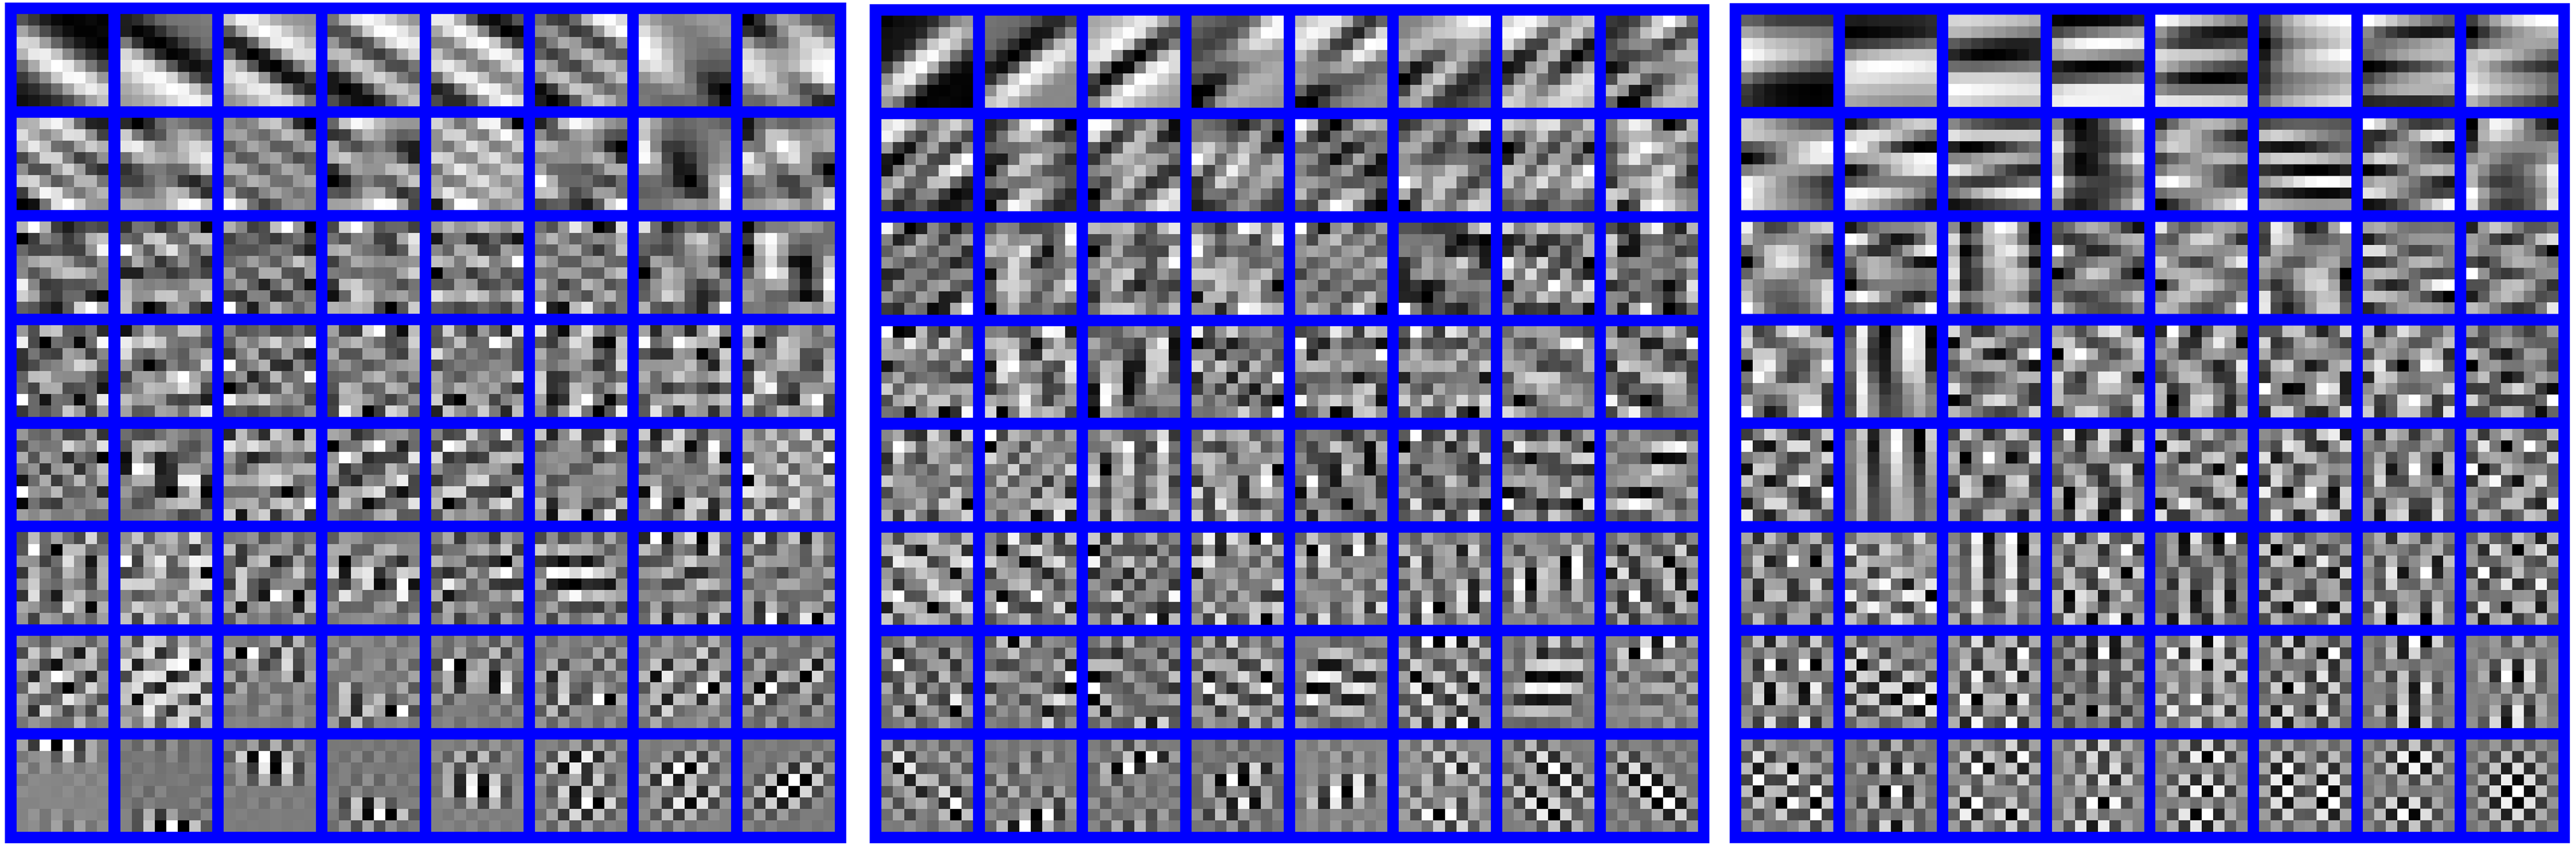
\includegraphics[width=1\linewidth]{images/pgpd/dics.png}
\caption{Eigenvectors of 3 Gaussian components from the learned PG-GMM, sorted by the values of corresponding eigenvalues.}
\label{fig4}
\end{figure}

For each patch $\bm{\overline{y}}_{m}$ in the PG $\bm{\overline{Y}}$, we propose to use $\bm{D}$ as the dictionary to sparsely encode $\bm{\overline{y}}_{m}$ as $\bm{\overline{y}}_{m}=\bm{D}\bm{\alpha}+\bm{v}$, where $\bm{\alpha}$ is the vector of sparse coding coefficients and $\bm{v}$ is the corrupted noise. Meanwhile, we propose to introduce a weighting vector $\bm{w}$ to weight the coding vector $\bm{\alpha}$ (we will see in (\ref{equ16}) that $\bm{w}$ is related to the eigenvalues in $\bm{\Lambda}$), resulting in the following simple but highly effective weighted sparse coding model:
\begin{equation}\label{equ11}
\min_{\bm{\alpha}}{\|\bm{\overline{y}}_{m}-\bm{D}\bm{\alpha}\|_{2}^{2}+\|\bm{w}^{T}\bm{\alpha}\|_{1}}.
\end{equation}

From the viewpoint of Maximum A-Posterior (MAP) estimation, the optimal solution of (\ref{equ11}) is $\hat{\bm{\alpha}} = \arg\max\nolimits_{\bm{\alpha}}\ln P(\bm{\alpha}|\bm{\overline{y}}_{m})$. By Bayes' formula, it is equivalent to
\begin{equation}\label{equ12}
\hat{\bm{\alpha}} = \arg\max\nolimits_{\bm{\alpha}}\{\ln P(\bm{\overline{y}}_{m}|\bm{\alpha})+\ln P(\bm{\alpha})\}.
\end{equation}
The log-likelihood term $\ln P(\bm{\overline{y}}_{m}|\bm{\alpha})$ is characterized by the statistics of noise $\bm{v}$, which is assumed to be white Gaussian with standard deviation $\sigma$. Hence, we have
\begin{equation}\label{equ13}
P(\bm{\overline{y}}_{m}|\bm{\alpha}) = \frac{1}{\sqrt{2\pi}\sigma}\exp(-\frac{1}{2\sigma^{2}}\|\bm{\overline{y}}_{m}-\bm{D}\bm{\alpha}\|_{2}^{2}).
\end{equation}
We assume that the sparse coding coefficients in $\bm{\alpha}$ follow i.i.d.\ Laplacian distribution.\ More specifically, for entry $\bm{\alpha}_{i}$, which is the coding coefficient of patch $\bm{\overline{y}}_{m}$ over the $i$th eigenvector in $\bm{D}$, we assume that it follows distribution $\frac{c}{\sqrt{2}\bm{\lambda}_{i}}\exp(-c\sqrt{2}|\bm{\alpha}_{i}|/\bm{\lambda}_{i})$, where $\bm{\lambda}_{i}=\bm{\Lambda}_{i}^{1/2}$ and $c$ is a constant. Note that we adjust the scale factor of the distribution by (square root of) the $i$th eigenvalue $\bm{\Lambda}_{i}$. This is because the larger the eigenvalue $\bm{\Lambda}_{i}$ is, the more important the $i$th eigenvector in $\bm{D}$ is, and hence the distribution of the coding coefficients over this eigenvector should have a longer tail (i.e., less sparse). Finally, we have
\begin{equation}\label{equ14}
P(\bm{\alpha})=\prod\nolimits_{i=1}^{p^{2}}\frac{c}{\sqrt{2}\bm{\lambda}_{i}}\exp(-\frac{c\sqrt{2}|\bm{\alpha}_{i}|}{\bm{\lambda}_{i}}).
\end{equation}
Putting (\ref{equ13}) and (\ref{equ14}) into (\ref{equ12}), we have
\begin{equation}\label{equ15}
\hat{\bm{\alpha}}=\arg\min\nolimits_{\bm{\alpha}}\|\bm{\overline{y}}_{m}-\bm{D}\bm{\alpha}\|_{2}^{2}+\sum_{i=1}^{p^{2}}\frac{c*2\sqrt{2}\sigma^{2}}{\bm{\lambda}_{i}}|\bm{\alpha}_{i}|.
\end{equation}
By comparing (\ref{equ15}) with (\ref{equ11}), we can see that the $i$th entry of the weighting vector $\bm{w}$ should be
\begin{equation}\label{equ16}
\bm{w}_{i} = c*2\sqrt{2}\sigma^{2}/(\bm{\lambda}_{i}+\varepsilon),
\end{equation}
where $\varepsilon$ is a small positive number to avoid dividing by zero.

With $\bm{w}$ determined by (\ref{equ16}), let's see what the solution of (\ref{equ11}) should be. Since the dictionary $\bm{D}$ is orthonormal, it is not difficult to find out that (\ref{equ11}) has a closed-form solution (detailed derivation can be found in the supplementary material):
\begin{equation}\label{equ17}
\hat{\bm{\alpha}}= \text{sgn}(\bm{D^{T}\overline{y}}_{m})\odot \text{max}(|\bm{D^{T}\overline{y}}_{m}|-\bm{w}/2,0),
\end{equation}
where $\text{sgn}(\bullet)$ is the sign function, $\odot$ means element-wise multiplication, and $|\bm{D^{T}\overline{y}}_{m}|$ is the absolute value of each entry of vector $|\bm{D^{T}\overline{y}}_{m}|$. The closed-form solution makes our weighted sparse coding process very efficient. 
\subsection{Denoising Algorithm}
With the solution $\hat{\bm{\alpha}}$ in (\ref{equ17}), the clean patch in a PG can be estimated as $\hat{\bm{x}}_{m}=\bm{D}\hat{\bm{\alpha}}+\bm{\mu}_{y}$. Then the clean image $\hat{\bm{x}}$ can be reconstructed by aggregating all the estimated PGs. In practice, we could perform the above denoising procedures for several iterations for better denoising outputs. In iteration $t$, we use the iterative regularization strategy \cite{osher2005iterative} to add back to the recovered image $\hat{\bm{x}}^{(t-1)}$ some estimation residual in iteration $t-1$. The standard deviation of noise in iteration $t$ is adjusted as $\sigma^{(t)} = \eta*\sqrt{\sigma^{2}-\|\bm{y}-\bm{y}^{(t-1)}\|_{2}^{2}}$, where $\eta$ is a constant. The proposed denoising algorithm is summarized in Algorithm 1 (Alg. 1).

In the proposed algorithm, there are $N$ PGs in an image and $M$ patches in each PG. Then the computational cost for Gaussian component selection is $O(p^{6}NMK)$.\ The cost for iterative regularization and noise estimation is negligible. The cost for closed-form weighted sparse coding is $O(p^{4}NM)$. Suppose that there are $T$ iterations, the overall complexity of our denoising algorithm is $O(p^{6}NMKT)$.
\begin{table}
\label{alg1}
\begin{tabular}{l}
\hline
\textbf{Alg. 1}: Patch Group Prior based Denoising (PGPD)
\\
\hline
\textbf{Input:} Noisy image $\bm{y}$, PG-GMM model
\\
1. Initialization: $\hat{\bm{x}}^{(0)}=\bm{y},\bm{y}^{(0)}=\bm{y}$;
\\
\textbf{for} $t = 1:IteNum$ \textbf{do}
\\
2. Iterative Regularization:
\\
\quad\quad\quad $\bm{y}^{(t)}=\hat{\bm{x}}^{(t-1)}+\delta(\bm{y}-\bm{y}^{(t-1)})$;
\\
3. Estimate the standard deviation of noise;
\\
\quad\textbf{for} each PG $\bm{Y}$ \textbf{do}
\\
4.\quad Calculate group mean $\bm{\mu}_{y}$ and form PG $\bm{\overline{Y}}$;
\\
5.\quad Gaussian component selection via (\ref{equ9});
\\
6.\quad Denoising by Weighted Sparse Coding (\ref{equ15});
\\
7.\quad Recover each patch in this PG via $\hat{\bm{x}}_{m}=\bm{D}\hat{\bm{\alpha}}+\bm{\mu}_{y}$;
\\
\quad\textbf{end for}
\\
8. Aggregate the recovered PGs to form the recovered
\\
\quad image $\hat{\bm{x}}^{(t)}$;
\\
\textbf{end for}
\\
\textbf{Output:} The recovered image $\hat{\bm{x}}^{(IteNum)}$.\\
\hline
\end{tabular}
\end{table}
%-------------------------------------------------------------------------
\section{Experiments}
In this section, we perform image denoising experiments on 20 widely used natural images (shown in Fig. \ref{fig5}). More experiments on the Berkeley Segmentation Data Set \cite{bsds} can be found in the supplementary file. As a common experimental setting in literature, additive white Gaussian noise with zero mean and standard deviation $\sigma$ is added to the image to test the performance of competing denoising methods. We call our method \textsl{PG Prior based Denoising} (PGPD) in the following experiments. The Matlab source code of our PGPD algorithm can be downloaded at \url{http://www4.comp.polyu.edu.hk/~cslzhang/code/PGPD.zip}.

\begin{figure}
    \centering
    \begin{subfigure}[b]{0.09\textwidth}
        \centering
        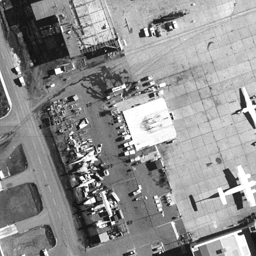
\includegraphics[width=1\textwidth]{images/pgpd/airfield.png}
    \end{subfigure}
    \hfill
    \begin{subfigure}[b]{0.09\textwidth}
        \centering
        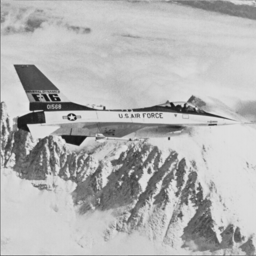
\includegraphics[width=1\textwidth]{images/pgpd/airplane.png}
    \end{subfigure}
    \hfill
    \begin{subfigure}[b]{0.09\textwidth}
        \centering
        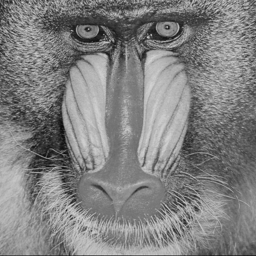
\includegraphics[width=1\textwidth]{images/pgpd/baboon.png}
    \end{subfigure}
    \hfill
    \begin{subfigure}[b]{0.09\textwidth}
        \centering
        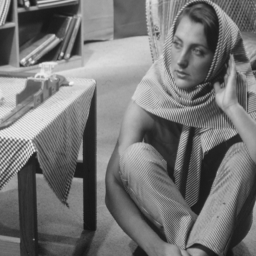
\includegraphics[width=1\textwidth]{images/pgpd/barbara.png}
    \end{subfigure}
    \hfill
    \begin{subfigure}[b]{0.09\textwidth}
        \centering
        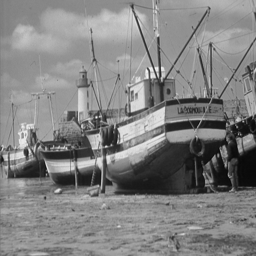
\includegraphics[width=1\textwidth]{images/pgpd/boat.png}
    \end{subfigure}
    \hfill
    \begin{subfigure}[b]{0.09\textwidth}
        \centering
        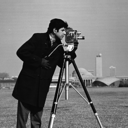
\includegraphics[width=1\textwidth]{images/pgpd/cameraman.png}
    \end{subfigure}
    \hfill
    \begin{subfigure}[b]{0.09\textwidth}
        \centering
        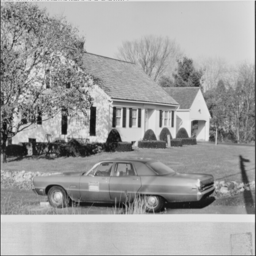
\includegraphics[width=1\textwidth]{images/pgpd/carhouse.png}
    \end{subfigure}
    \hfill
    \begin{subfigure}[b]{0.09\textwidth}
        \centering
        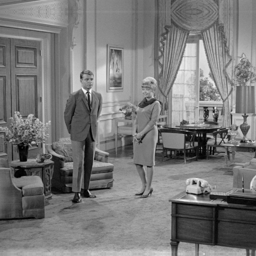
\includegraphics[width=1\textwidth]{images/pgpd/couple.png}
    \end{subfigure}
    \hfill
    \begin{subfigure}[b]{0.09\textwidth}
        \centering
        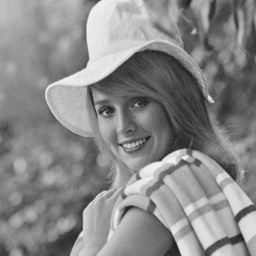
\includegraphics[width=1\textwidth]{images/pgpd/elaine.png}
    \end{subfigure}
    \hfill
    \begin{subfigure}[b]{0.09\textwidth}
        \centering
        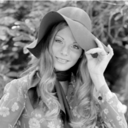
\includegraphics[width=1\textwidth]{images/pgpd/hat.png}
    \end{subfigure}
    \hfill
    \begin{subfigure}[b]{0.09\textwidth}
        \centering
        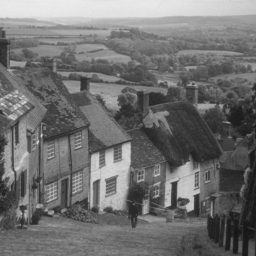
\includegraphics[width=1\textwidth]{images/pgpd/hill.png}
    \end{subfigure}
    \hfill
    \begin{subfigure}[b]{0.09\textwidth}
        \centering
        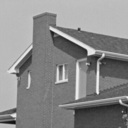
\includegraphics[width=1\textwidth]{images/pgpd/house.png}
    \end{subfigure}
    \hfill
    \begin{subfigure}[b]{0.09\textwidth}
        \centering
        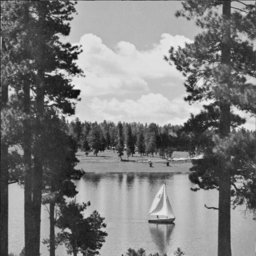
\includegraphics[width=1\textwidth]{images/pgpd/lake.png}
    \end{subfigure}
    \hfill
    \begin{subfigure}[b]{0.09\textwidth}
        \centering
        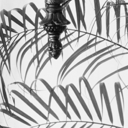
\includegraphics[width=1\textwidth]{images/pgpd/leaves.png}
    \end{subfigure}
    \hfill
    \begin{subfigure}[b]{0.09\textwidth}
        \centering
        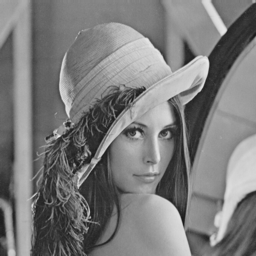
\includegraphics[width=1\textwidth]{images/pgpd/lena.png}
    \end{subfigure}
    \hfill
    \begin{subfigure}[b]{0.09\textwidth}
        \centering
        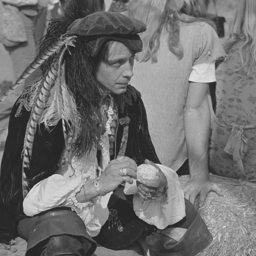
\includegraphics[width=1\textwidth]{images/pgpd/man.png}
    \end{subfigure}
    \hfill
    \begin{subfigure}[b]{0.09\textwidth}
        \centering
        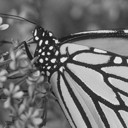
\includegraphics[width=1\textwidth]{images/pgpd/monarch.png}
    \end{subfigure}
    \hfill
    \begin{subfigure}[b]{0.09\textwidth}
        \centering
        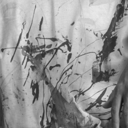
\includegraphics[width=1\textwidth]{images/pgpd/paint.png}
    \end{subfigure}
    \hfill
    \begin{subfigure}[b]{0.09\textwidth}
        \centering
        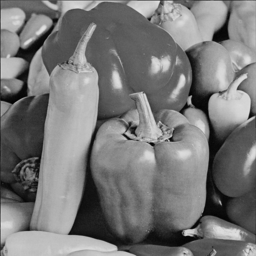
\includegraphics[width=1\textwidth]{images/pgpd/peppers.png}
    \end{subfigure}
    \hfill
    \begin{subfigure}[b]{0.09\textwidth}
        \centering
        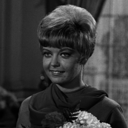
\includegraphics[width=1\textwidth]{images/pgpd/zelda.png}
    \end{subfigure}
    \caption{The 20 widely used test images.}
    \label{fig5}
\end{figure}


\subsection{Implementation Details}
Our proposed PGPD method contains two stages, the prior learning stage and the denoising stage. In the PG-GMM learning stage, there are 4 parameters: $p$, $M$, $W$ and $K$. The patch size ($p\times p$) is set as $p = 6$ for $0 < \sigma \le 20$, $p = 7$ for $20 < \sigma \le 30$, $p = 8$ for $30 < \sigma \le 50$, and $p=9$ for $50 < \sigma \le 100$. The window size ($W$) for PG searching is set to $W = 31$. The number ($M$) of patches in a PG is set to $M=10$. The number ($K$) of Gaussian components is set to $K=64$ for $p=6$ and $K=32$ otherwise. We extracted about one million PGs from the Kodak PhotoCD Dataset to train the PG-GMM. 

In the denoising stage, there are 3 parameters:\ $c$, $\delta$, and $\eta$.\ In our implementation, ($c$, $\delta$, $\eta$) are set to $(0.33,0.10,0.79)$, $(0.29,0.09,0.73)$, $(0.19,0.08,0.89)$, $(0.15,0.07,0.98)$, $(0.12,0.06,1.05)$, $(0.09,0.05,1.15)$, $(0.06,0.05,1.30)$ when $\sigma=10,20,30,40,50,75,100$, respectively. In addition, on all noise levels we stop Algorithm 1 in 4 iterations.

\subsection{Comparison with Patch Prior based Denoising}
In this section, we compare the PSNR and visual quality of denoised images by the \textsl{Patch Prior based Denoising} (PPD) method and the \textsl{Patch Group Prior based Denoising} (PGPD) method. As can be seen from Table \ref{tab1} and Figures \ref{fig1}-\ref{fig4}, PGPD is much better than PPD both quantitatively and qualitatively. This validates the effectiveness of our learned PG based NSS prior. In the following sections, we will omit the results of the PPD method.
\begin{table}
\begin{adjustwidth}{-3cm}{}
\scriptsize
\caption{PSNR(dB) results of PPD and PGPD on the 20 natural images.}
\label{tab1}
\centering
\begin{tabular}{|c||c|c||c|c||c|c||c|c||c|c||c|c||c|c|}
\hline
&\multicolumn{2}{c||}{ $\sigma = 10$}&\multicolumn{2}{c||}{ $\sigma = 20$}&\multicolumn{2}{c||}{ $\sigma = 30$}
&\multicolumn{2}{c||}{ $\sigma = 40$}&\multicolumn{2}{c||}{ $\sigma = 50$}&\multicolumn{2}{c||}{ $\sigma = 75$}
&\multicolumn{2}{c|}{ $\sigma = 100$}
\\
\hline
\hline
Images&\textbf{PPD}&\textbf{PGPD}&\textbf{PPD}&\textbf{PGPD}&\textbf{PPD}&\textbf{PGPD}&\textbf{PPD}&\textbf{PGPD}&\textbf{PPD}
&\textbf{PGPD}&\textbf{PPD}&\textbf{PGPD}&\textbf{PPD}&\textbf{PGPD}
\\
\hline
Airfield&31.02 &31.18  &27.97&28.19  &26.33& 26.46   &25.20 & 25.30  & 24.33 & 24.44  &22.69 &22.90   &21.54&21.82 
\\
\hline
Airplane&35.87 &36.00     &32.59&32.69   &30.62&30.80 &29.21&29.44  &28.10& 28.38    &25.90& 26.39  &24.35 &25.01
\\
\hline
Baboon&30.46&30.55   &26.54&26.67  &24.54 & 24.63 & 23.23&23.39  & 22.30&22.47    &20.71 & 21.09   &19.99 &20.38
\\
\hline 
Barbara&33.96&34.74    &30.24&31.40 & 27.97 & 29.38 & 26.29 & 27.97  &24.94 & 26.81  &22.84 &24.84   &22.04&23.48
\\
\hline
Boat&33.58&33.77     &30.58&30.82    & 28.80 &  29.05  &27.51 & 27.82   & 26.52 &  26.85   & 24.72 &25.19  & 23.56&24.06       
\\
\hline
C. Man&33.91&34.14     &30.12&30.35  & 28.25& 28.53  & 27.05& 27.33  & 26.13 & 26.46  &24.36 &24.64    &22.80 &23.23 
\\
\hline
Carhouse&34.35 &34.47     &30.61&30.73   &28.62 & 28.80  & 27.29&27.51  &26.27 &26.53  &24.44&24.85    &23.21&23.67
\\
\hline
Couple &33.78&34.03       &30.47&30.71  & 28.54 & 28.84 & 27.16 & 27.53   &26.07 & 26.50  &24.22 &24.70   &23.12 &23.55
\\
\hline
Elaine&32.73&32.98   &31.21&31.32    &30.24& 30.37   &29.42&29.62   &28.69 &28.90   &27.26&27.47   &26.17&26.27
\\
\hline
Hat&35.44&35.44      &31.42 &31.44  & 29.05&29.31   &27.43&27.90  & 26.28 &26.76  &24.19 & 24.79    &22.86&23.45
\\
\hline
Hill&33.38&33.58     &30.41&30.66   &28.85 & 29.09   &27.76 & 28.06  & 26.91 &27.22  &25.34 & 25.73   &24.36 &24.66
\\
\hline
House&35.61&36.56      &33.18&33.85   & 31.62& 32.24  &30.32 &31.02  & 29.17 &29.93   &26.81 & 27.81  & 25.13&26.17  
\\
\hline
Lake&32.86&32.98     &30.00&30.09   &28.30 &28.38   &27.03 & 27.15  & 26.05 &26.20   &24.19 &24.49    &22.94 &23.36
\\
\hline
Leaves&33.87& 34.45     &29.84&30.46    &27.51 &27.99  & 25.88 & 26.29  &24.56 &25.03   &21.94& 22.61   &19.77&20.95
\\
\hline  
Lena&35.59&35.81     &32.75&32.94  &30.98 &31.27  &29.67 &30.10   &28.61 & 29.11   &26.68 &  27.40      &25.41 &26.09
\\
\hline
Man&33.91&33.98      &30.52&30.60  & 28.72 & 28.86   &27.53 & 27.73   &26.63 &  26.86  &25.01& 25.36     &24.00 &24.33 
\\
\hline
Monarch&34.27&34.53    &30.40&30.68   & 28.27&28.49    &26.81 &27.02  &25.66 & 26.00  &23.51 & 24.00       &21.89 &22.56 
\\
\hline
Paint &34.16&34.31    &30.52&30.62   &28.39 &28.42   & 26.88 & 26.94  &25.70 & 25.82 &23.50& 23.89  &22.05&22.65
\\
\hline
Peppers&34.71&34.82    & 32.61&32.66   &31.13 & 31.25 &29.95  & 30.18  &28.99 & 29.22  &27.04&  27.42    &25.45 &25.94
\\  
\hline
Zelda&35.50&35.51    &32.21&32.21  & 30.35 &30.43   &29.07 &29.23   & 28.06& 28.24  &26.37& 26.56     &25.28&25.41
\\
\hline
\textbf{Average}&33.95&34.19    &30.71&30.95   & 28.85 & 29.13   &27.53&27.88   & 26.50 & 26.89  &24.59 &25.11  &23.30&23.85       
\\
\hline
\end{tabular}
\end{adjustwidth}
\end{table}

\begin{figure}
    \centering
    \begin{subfigure}[t]{0.24\textwidth}
        \centering
        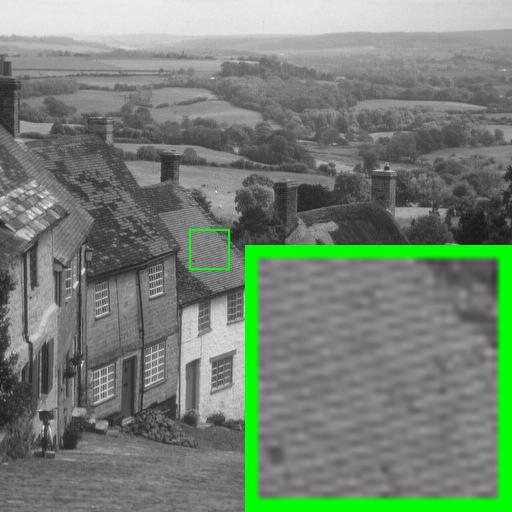
\includegraphics[width=1\textwidth]{images/pgpd/pgdpd/br_hill.jpg}
	   \caption{Clean}
    \end{subfigure}
    \hfill
    \begin{subfigure}[t]{0.24\textwidth}
        \centering
        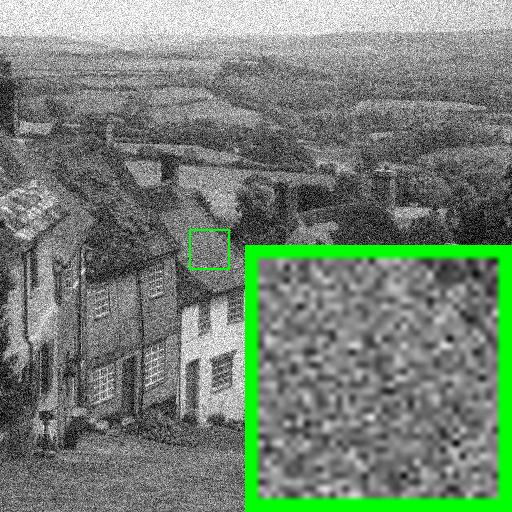
\includegraphics[width=1\textwidth]{images/pgpd/pgdpd/br_30_hill.jpg}
		\caption{Noisy: 18.59}
    \end{subfigure}
    \hfill
    \begin{subfigure}[t]{0.24\textwidth}
        \centering
        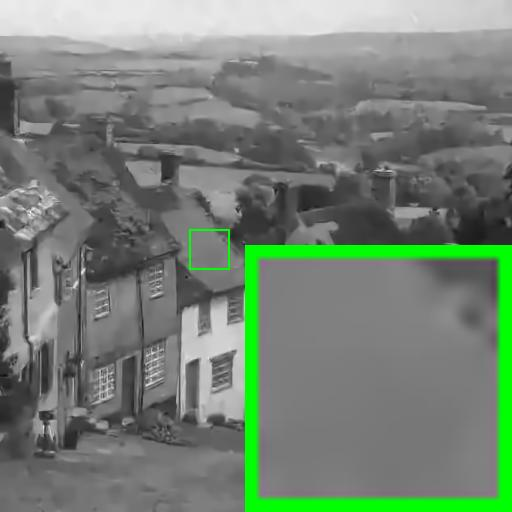
\includegraphics[width=1\textwidth]{images/pgpd/pgdpd/br_GMM65_30_hill.jpg}
		\caption{PPD: 28.85}
    \end{subfigure}
    \hfill
    \begin{subfigure}[t]{0.24\textwidth}
        \centering
        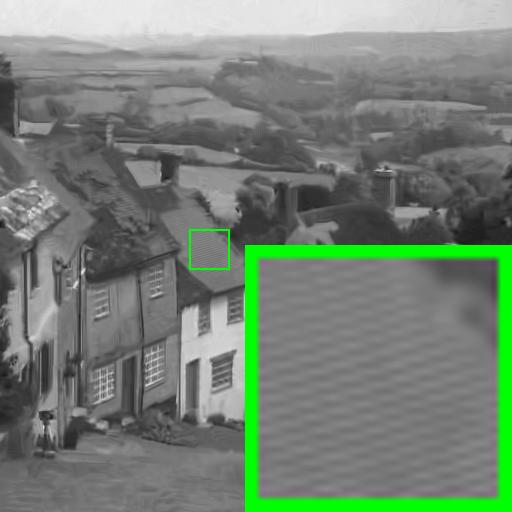
\includegraphics[width=1\textwidth]{images/pgpd/pgdpd/br_our_30_hill.jpg}
		\caption{PGPD: 29.09}
    \end{subfigure}
    \caption{Denoised images and PSNR (dB) results of \textsl{Hill} by the PPD method and PGPD method (the standard deviation of noise is $\sigma=30$).}
    \label{fig6}
\end{figure}


\begin{figure}
    \centering
    \begin{subfigure}[t]{0.24\textwidth}
        \centering
        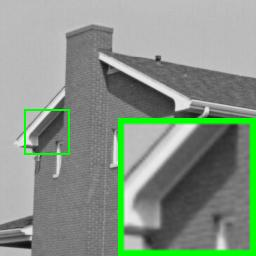
\includegraphics[width=1\textwidth]{images/pgpd/pgdpd/br_house.jpg}
	   \caption{Clean}
    \end{subfigure}
    \hfill
    \begin{subfigure}[t]{0.24\textwidth}
        \centering
        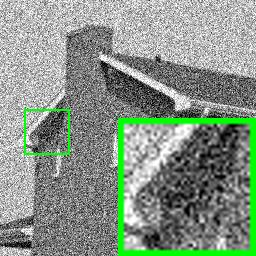
\includegraphics[width=1\textwidth]{images/pgpd/pgdpd/br_40_house.jpg}
		\caption{Noisy: 16.06}
    \end{subfigure}
    \hfill
    \begin{subfigure}[t]{0.24\textwidth}
        \centering
        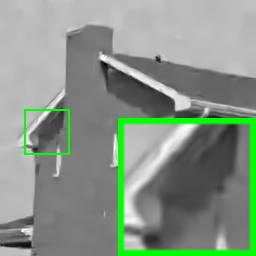
\includegraphics[width=1\textwidth]{images/pgpd/pgdpd/br_GMM65_40_house.jpg}
		\caption{PPD: 30.32}
    \end{subfigure}
    \hfill
    \begin{subfigure}[t]{0.24\textwidth}
        \centering
        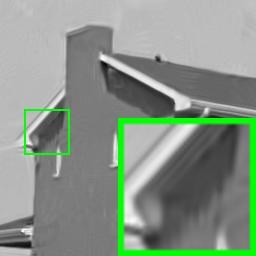
\includegraphics[width=1\textwidth]{images/pgpd/pgdpd/br_our_40_house.jpg}
		\caption{PGPD: 31.02}
    \end{subfigure}
    \caption{Denoised images and PSNR (dB) results of \textsl{House} by the PPD method and PGPD method (the standard deviation of noise is $\sigma=40$).}
    \label{fig6}
\end{figure}


\begin{figure}
    \centering
    \begin{subfigure}[t]{0.24\textwidth}
        \centering
        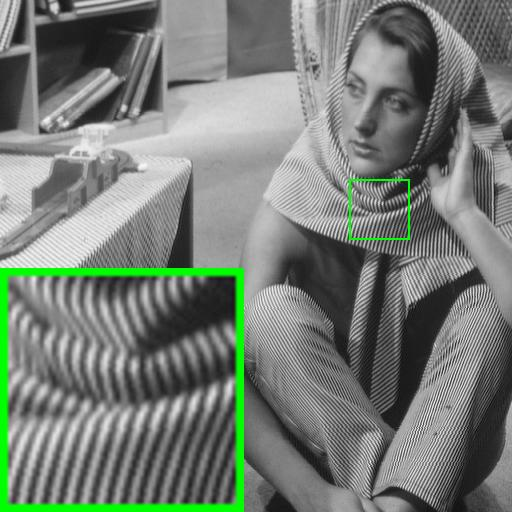
\includegraphics[width=1\textwidth]{images/pgpd/pgdpd/br_barbara.jpg}
	   \caption{Clean}
    \end{subfigure}
    \hfill
    \begin{subfigure}[t]{0.24\textwidth}
        \centering
        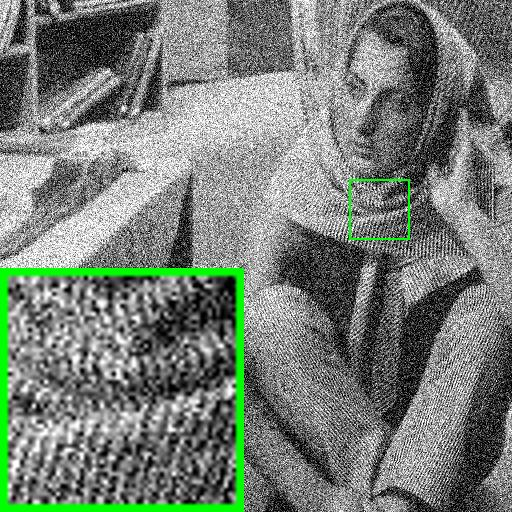
\includegraphics[width=1\textwidth]{images/pgpd/pgdpd/br_50_barbara.jpg}
		\caption{Noisy: 14.16}
    \end{subfigure}
    \hfill
    \begin{subfigure}[t]{0.24\textwidth}
        \centering
        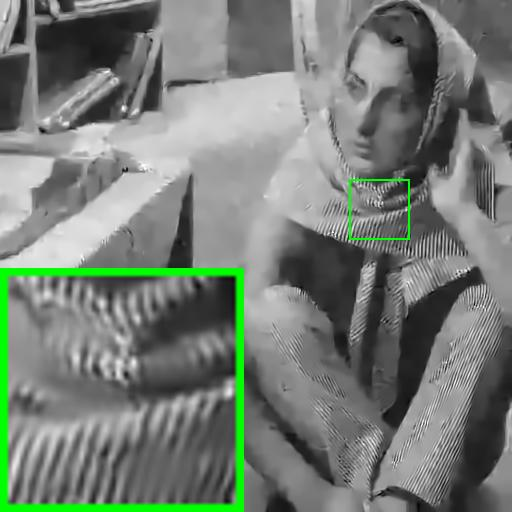
\includegraphics[width=1\textwidth]{images/pgpd/pgdpd/br_GMM65_50_barbara.jpg}
		\caption{PPD: 24.94}
    \end{subfigure}
    \hfill
    \begin{subfigure}[t]{0.24\textwidth}
        \centering
        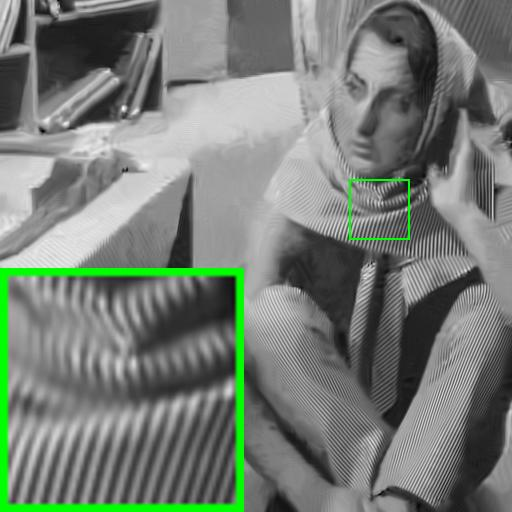
\includegraphics[width=1\textwidth]{images/pgpd/pgdpd/br_our_50_barbara.jpg}
		\caption{PGPD: 26.81}
    \end{subfigure}
    \caption{Denoised images and PSNR (dB) results of \textsl{Barbara} by the PPD method and PGPD method (the standard deviation of noise is $\sigma=50$).}
    \label{fig6}
\end{figure}


\begin{figure}
    \centering
    \begin{subfigure}[t]{0.24\textwidth}
        \centering
        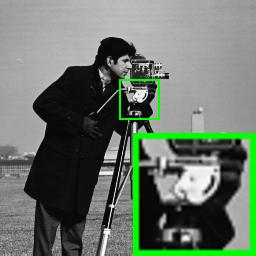
\includegraphics[width=1\textwidth]{images/pgpd/pgdpd/br_cameraman.jpg}
	   \caption{Clean}
    \end{subfigure}
    \hfill
    \begin{subfigure}[t]{0.24\textwidth}
        \centering
        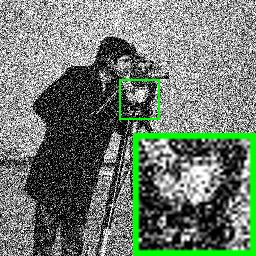
\includegraphics[width=1\textwidth]{images/pgpd/pgdpd/br_75_cameraman.jpg}
		\caption{Noisy: 10.60}
    \end{subfigure}
    \hfill
    \begin{subfigure}[t]{0.24\textwidth}
        \centering
        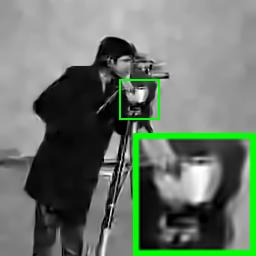
\includegraphics[width=1\textwidth]{images/pgpd/pgdpd/br_GMM65_75_cameraman.jpg}
		\caption{PPD: 24.36}
    \end{subfigure}
    \hfill
    \begin{subfigure}[t]{0.24\textwidth}
        \centering
        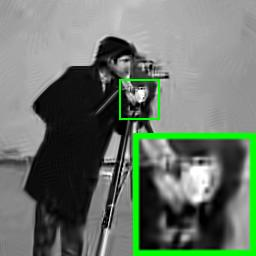
\includegraphics[width=1\textwidth]{images/pgpd/pgdpd/br_our_75_cameraman.jpg}
		\caption{PGPD:24.64}
    \end{subfigure}
    \caption{Denoised images and PSNR (dB) results of \textsl{Cameraman} by the PPD method and PGPD method (the standard deviation of noise is $\sigma=75$).}
    \label{fig6}
\end{figure}


\subsection{Comparison With the State-of-the-art Methods}
We compare the proposed PGPD algorithm with BM3D \cite{bm3d}, EPLL \cite{epll}, LSSC \cite{lssc}, NCSR \cite{ncsr}, and WNNM \cite{wnnm}, which represent the state-of-the-arts of modern image denoising techniques and all of them exploit image NSS. The source codes of all competing algorithms are downloaded from the authors' websites and we use the default parameter settings.  

To more clearly demonstrate the effectiveness of PG based NSS prior learning, we also compare with an extreme case of PGPD, i.e., letting $M=1$ in the PG-GMM learning stage\footnote{Since there is only 1 patch in the PG, the group mean vector cannot be subtracted and we subtract the mean value of the patch from it.}. Clearly, this reduces to a patch based prior learning scheme and no NSS prior will be learned. We call this extreme case as \textsl{Patch Prior based Denoising} (PPD).  The number of Gaussian components in PPD is set to 64, and the weighted sparse coding framework in it is the same as that in PGPD. All the other parameters in PPD are tuned to achieve its best performance.
\subsection{Results and Discussions}
We evaluate the competing methods from three aspects: PSNR, Speed, and Visual Quality.

\textbf{PSNR}. In Table \ref{tab1}, we present the PSNR results on four noise levels $\sigma=30,40,50,75$. The results on noise levels $\sigma=10,20,100$ can be found in the supplementary material. From Table \ref{tab1}, we have several observations. Firstly, PGPD achieves much better PSNR results than PPD. The improvements are 0.24$\sim$0.52dB on average. This clearly demonstrates the effectiveness of PG-GMM in NSS prior learning. Secondly, PGPD has higher PSNR values than BM3D, LSSC, EPLL and NCSR, and is only slightly inferior to WNNM. However, PGPD is much more efficient than WNNM (see next paragraph). This validates the strong ability of PG based NSS prior in image denoising. 

\textbf{Speed}. Efficiency is another important factor to evaluate an algorithm. We then compare the speed of all competing methods. All experiments are run under the Matlab2014b environment on a machine with Intel(R) Core(TM) i7-4770K CPU of 3.50GHz and 12.0 GB RAM. The run time (s) of competing methods on the test images is shown in Table \ref{tab2}.\ One can easily see that BM3D is the fastest method. The proposed PGPD is the second fastest, and it is much faster than the other methods. For a $256\times256$ image, BM3D costs about 0.8s while PGPD costs about 10s. However, please note that BM3D is implemented with compiled C++ mex-function and with parallelization, while PGPD is implemented purely in Matlab. EPLL is about 4 times slower than PGPD. Both LSSC and NCSR are very slow since they need to train online dictionary.\ Though WNNM has the highest PSNR, it suffers from huge computational cost due to the many online SVD operations. It is 10$\sim$16 times slower than PGPD. 

\textbf{Visual Quality}. Considering that human subjects are the ultimate judge of the image quality, the visual quality of denoised images is also critical to evaluate a denoising algorithm. Fig. \ref{fig6} and Fig. \ref{fig7} show the denoised images of \textsl{Airplane} and \textsl{Cameraman} by the competing methods, respectively. Due to the page limit, the results of PPD are not shown here, and more visual comparisons can be found in the supplementary file.\ We can see that BM3D tends to over-smooth the image, while EPLL, LSSC, NCSR and WNNM are likely to generate artifacts when noise is high. Owe to the learned NSS prior, the proposed PGPD method is more robust against artifacts, and it preserves edge and texture areas much better than the other methods. For example, in image \textsl{Airplane}, PGPD reconstructs the numbers ``01568'' more clearly than all the other methods including WNNM. In image \textsl{Cameraman}, PGPD recoveries more faithfully the fine structures of the camera area. 

In summary, the proposed PGPD method demonstrates powerful denoising ability quantitatively and qualitatively, and it is highly efficient.
\begin{table}[t]
\caption{PSNR(dB) results of different denoising algorithms on 20 natural images.}
\label{tab1}
\begin{adjustwidth}{-3cm}{}
\begin{center}
\renewcommand\arraystretch{1.0}
\scriptsize
\begin{tabular}{|c||c|c|c|c|c|c||c|c|c|c|c|c|}
\hline
&\multicolumn{6}{c||}{ $\sigma = 10$}&\multicolumn{6}{c|}{ $\sigma = 20$}
\\
\hline
\hline
Images&\textbf{BM3D}&\textbf{LSSC}&\textbf{EPLL}&\textbf{NCSR}&\textbf{WNNM}&\textbf{PGPD}
&\textbf{BM3D}&\textbf{LSSC}&\textbf{EPLL}&\textbf{NCSR}&\textbf{WNNM}&\textbf{PGPD} 
\\
\hline
Airfield &31.32&31.51&31.37&31.40 &31.47 &31.18    &28.13&28.48 &28.18&28.07&28.40&28.19 
\\
\hline
Airplane &35.97 &36.05&35.92&36.04&36.26 &36.00  &32.63&32.57 &32.64&32.69&32.91&32.69 
\\
\hline
 Baboon &30.58&30.67&30.62&30.61&30.79&30.55     &26.61&26.75 &26.71&26.64&26.84&26.67
\\
\hline 
 Barbara &34.98&34.99&33.65 &35.01&35.51&34.74    &31.78&31.60 &29.85 &31.78 &32.19&31.40
\\
\hline
 Boat &33.92&34.03 &33.67&33.92&34.09&33.77     &30.88&30.92&30.71&30.79&31.01&30.82
\\
\hline
 C. Man &34.18 &34.24&34.05 &34.18&34.44&34.14      &30.48 &30.59 &30.38 &30.47&30.75&30.35 
\\
\hline
 Carhouse &34.45&34.52&34.32 &34.51&34.70 &34.47   &30.74&30.77&30.66&30.79&30.90&30.73
\\
\hline
 Couple &34.04&34.01&33.88&34.00&34.14&34.03    &30.76 &30.74&30.60&30.60&30.82&30.71 
\\
\hline
 Elaine &33.36 &34.36&32.90&33.83&33.76&32.98    &31.48 &31.74 &31.25&31.47&31.44&31.32
\\
\hline
 Hat &35.40 &35.56&35.23&35.45&35.75&35.44    &31.55 &31.48&31.41&31.48&31.66 &31.44
\\
\hline
 Hill &33.62 &33.68&33.49&33.69&33.79&33.58      &30.72&30.73 &30.50&30.65&30.81&30.66
\\
\hline
 House &36.71 &36.95&35.75&36.79&36.95&36.56     &33.77&34.11 &33.12&33.87&34.01&33.85
\\
\hline
 Lake &33.03 &33.23&33.00&33.10 &33.21&32.98      &30.05&30.15&30.09 &30.05&30.29&30.09
\\
\hline
 Leaves &34.04&34.52&33.39&34.52&35.20& 34.45   &30.09&30.46&29.55&30.45 &31.10&30.46 
\\
\hline
 Lena &35.93 &35.85&35.62&35.85&36.06&35.81    &33.05 &32.89&32.74&32.95&33.12&32.94  
\\
\hline
 Man &33.98 &34.10&34.01&34.05&34.23&33.98    &30.59&30.72&30.68&30.59 &30.77&30.60   
\\
\hline
 Monarch &34.12&34.44&34.36 &34.51&35.03&34.53     &30.35 &30.59&30.60 &30.62&31.11&30.68
\\
\hline
 Paint &34.00&34.35&34.09&34.15&34.50&34.31     &30.36&30.59 &30.50&30.33&30.77&30.62  
\\
\hline
 Peppers &35.01&35.13&34.83 &35.03&35.06&34.82    &32.76&32.61 &32.61&32.66&32.81&32.66 
\\
\hline
 Zelda &35.62&35.54&35.57 &35.49&35.69&35.51     &32.29 &32.06 &32.29&32.10&32.30 &32.21
\\
\hline
 \textbf{Average} &34.21&34.39&33.99 &34.31&34.53&34.19  &30.95 &31.03 &34.75&30.95&31.20&30.95   
\\
\hline
\hline
&\multicolumn{6}{c||}{ $\sigma = 30$}&\multicolumn{6}{c|}{ $\sigma = 40$}
\\
\hline
\hline
Images&\textbf{BM3D}&\textbf{LSSC}&\textbf{EPLL}&\textbf{NCSR}&\textbf{WNNM}&\textbf{PGPD}
&\textbf{BM3D}&\textbf{LSSC}&\textbf{EPLL}&\textbf{NCSR}&\textbf{WNNM}&\textbf{PGPD} 
\\
\hline
Airfield& 26.41 & 26.68 & 26.52  &  26.36  & 26.67 & 26.46     & 25.10 &  25.51  & 25.36 & 25.07 & 25.48 & 25.30 
\\
\hline
Airplane&  30.71  & 30.62  &  30.68  &  30.70 & 30.97 & 30.80    & 29.20 & 29.21  & 29.28 & 29.28 & 29.58 & 29.44
\\
\hline
 Baboon & 24.57   & 24.78  & 24.70   & 24.63  & 24.85 & 24.63   &  23.11 &  23.51  & 23.35 & 23.28 & 23.58 & 23.39   
\\
\hline 
 Barbara & 29.81  & 29.60 & 27.64 & 29.62 & 30.31 & 29.38   &  27.99 & 28.17 & 26.06 & 28.20 & 28.76 & 27.97
\\
\hline
 Boat & 29.12  & 29.06  & 28.97 & 28.94 & 29.24 &  29.05   &  27.74& 27.77  &  27.72 & 27.65 &27.96  & 27.82    
\\
\hline
 C. Man& 28.64 & 28.63 & 28.40  & 28.58 & 28.80& 28.53     & 27.18& 27.34  & 27.10 &27.12  &27.47 & 27.33
\\
\hline
 Carhouse& 28.78 & 28.79   & 28.70    & 28.72 & 28.94 & 28.80   & 27.38 &  27.49 & 27.38 & 27.40 & 27.58 & 27.51
\\
\hline
 Couple & 28.87  & 28.76  & 28.69 & 28.57 & 28.98 & 28.84    & 27.48 & 27.41 &  27.34  & 27.24 & 27.62 & 27.53   
\\
\hline
 Elaine& 30.45 & 30.54 & 30.26   &  30.26  & 30.46 & 30.37    &29.52 & 29.55 & 29.46 & 29.59 & 29.60 &29.62   
\\
\hline
 Hat& 29.37 & 29.22  & 29.22   &  29.16  & 29.44  &29.31    & 27.74 & 27.60 &  27.73  &  27.66 & 27.85  &27.90   
\\
\hline
 Hill & 29.16 & 29.09 & 28.94 & 28.97 & 29.25 & 29.09    & 27.99 & 28.00 & 27.86 & 27.83 & 28.12 & 28.06 
\\
\hline
 House& 32.09 & 32.40  & 31.48  & 32.07 & 32.52 & 32.24    & 30.65  & 31.10 & 30.20 & 30.80  & 31.31 &31.02    
\\
\hline
 Lake   & 28.34 & 28.36  & 28.41   & 28.31   &  28.59 &28.38    & 26.98  & 27.13 &27.19  & 26.99 &27.34 & 27.15  
\\
\hline
 Leaves & 27.81 & 27.65& 27.36 & 28.14 & 28.60 &27.99     & 25.69 & 26.04 & 25.80 &26.24 & 26.95 & 26.29  
\\
\hline
 Lena& 31.26 & 31.18  & 30.98 &  31.06& 31.43 &31.27     & 29.86& 29.91 & 29.69& 29.92 & 30.11 &30.10   
\\
\hline
 Man& 28.86 & 28.87 & 28.87 & 28.78 & 29.00 & 28.86    & 27.65  & 27.64 & 27.68& 27.54 &27.80 & 27.73     
\\
\hline
 Monarch& 28.36 & 28.20 & 28.50 & 28.46 & 28.91 &28.49    &   26.72  & 26.87 &27.05  & 26.85 & 27.47 &27.02    
\\
\hline
 Paint & 28.29 & 28.29 & 28.45  &  28.10  & 28.58 &28.42    &  26.69 &  26.77 & 27.00  & 26.50 & 27.10 & 26.94 
\\
\hline
 Peppers & 31.26 & 31.17 & 31.10 & 31.11  & 31.38 & 31.25   &   29.97  & 30.00&  29.93 &  30.07 & 30.18 & 30.18    
\\
\hline
 Zelda & 30.45 & 30.27  & 30.44  &  30.16  & 30.48 &30.43    & 29.10&28.91 &29.18  & 28.94 & 29.12 &29.23   
\\
\hline
 \textbf{Average} &  29.13 & 29.11  &  28.92 & 29.03  & 29.37 & 29.13   &27.69&27.80 & 27.62& 27.71&28.05 &27.88     
\\
\hline
\hline
&\multicolumn{6}{c||}{ $\sigma = 50$}&\multicolumn{6}{c|}{ $\sigma = 75$}
\\
\hline
\hline
Images&\textbf{BM3D}&\textbf{LSSC}&\textbf{EPLL}&\textbf{NCSR}&\textbf{WNNM}&\textbf{PGPD}
&\textbf{BM3D}&\textbf{LSSC}&\textbf{EPLL}&\textbf{NCSR}&\textbf{WNNM}&\textbf{PGPD} 
\\
\hline
 Airfield & 24.20 & 24.58 & 24.46  &24.18 & 24.51 & 24.44    & 22.71 & 22.85 & 22.85 & 22.57 &22.94 &22.90 
\\
\hline
 Airplane & 28.24 & 28.15 & 28.19 & 28.18 &  28.55 & 28.38     & 26.40 & 26.16 & 26.14  & 26.10 &  26.68 & 26.39
\\
\hline
 Baboon & 22.35  & 22.60 & 22.35 & 22.43  & 22.73 &22.47     &  21.11&  21.18  & 20.85  & 21.03  & 21.36 & 21.09
\\
\hline
 Barbara & 27.23  & 27.03  & 24.83  & 26.99 &  27.79 & 26.81    & 25.12  & 25.01  & 22.94   &  24.72& 25.81 &24.84
\\
\hline
  Boat& 26.78 & 26.77  & 26.74  & 26.67 & 26.97 &  26.85   & 25.12 & 25.03 & 25.01 &  24.87&  25.29 &25.19         
\\
\hline
 C. Man   & 26.12 & 26.35   & 26.10 & 26.15 & 26.42 & 26.46   & 24.33 & 24.41 &  24.29  & 24.22 &  24.55 &24.64     
\\
\hline
 Carhouse  & 26.53 & 26.48  &  26.39   & 26.41 & 26.67 &26.53   &  24.89 & 24.85  &  24.65  & 24.53  &25.04 &24.85
\\
\hline
 Couple & 26.46 & 26.35  & 26.30 & 26.19 &  26.65 & 26.50   & 24.70 & 24.51 & 24.51 & 24.33 & 24.85 &24.70   
\\
\hline
 Elaine &  28.94 & 28.75 & 28.77   & 28.85 & 28.97 &28.90    &   27.41  & 27.27 & 27.38  &  27.16 &27.53 &27.47   
\\
\hline
 Hat  &  26.77 & 26.41 & 26.62  & 26.51 & 26.78 &26.76      &   24.77  & 24.31  & 24.65   &  24.48 &24.77 & 24.79
\\
\hline
 Hill  & 27.19 & 27.14  & 27.04 & 26.99   &27.34 &27.22     & 25.68 & 25.57 & 25.60 &  25.40 & 25.88  & 25.73
\\
\hline
 House  & 29.69 & 29.99  & 29.12  & 29.62  & 30.32 &29.93     & 27.51 & 27.75  &  27.09 &  27.22 & 28.25 & 27.81    
\\
\hline
 Lake   &  26.13  & 26.15  & 26.24  &  26.02  & 26.41 &26.20    & 24.49 & 24.25 & 24.50 & 24.26 &24.66 &24.49   
\\
\hline
 Leaves   & 24.68 & 24.78   & 24.55  & 24.96 & 25.47 &25.03     & 22.49  & 22.17 & 22.12 &  22.60 & 23.06 & 22.61
\\
\hline
 Lena  & 29.05 & 28.95 & 28.68 & 28.90 &  29.25 & 29.11      & 27.26 & 27.22 &  26.88 & 27.00 & 27.54 &  27.40   
\\
\hline
 Man   & 26.81 & 26.72    & 26.79 & 26.67 &  26.94 & 26.86   & 25.32 & 25.10  & 25.26  & 25.10 &  25.42 & 25.36      
\\
\hline
 Monarch  & 25.82 & 25.88 & 25.94 & 25.76 & 26.31 & 26.00   & 23.91 & 23.66  &  23.88   &  23.67& 24.31 & 24.00   
\\
\hline
 Paint & 25.67 & 25.59 & 25.87 & 25.36 &25.98 & 25.82     &  23.80 & 23.52 &  23.88 & 23.44 &24.07 & 23.89  
\\
\hline
 Peppers & 29.12 & 29.06 & 28.98 & 29.07 & 29.34 & 29.22     & 27.28 & 27.14 &  27.15 & 26.96 &  27.55   & 27.42
\\
\hline
 Zelda  & 28.25 & 27.90 & 28.22 & 27.97 & 28.21 & 28.24       & 26.60 & 26.09 &  26.55  & 26.21  & 26.44 & 26.56
\\
\hline
 \textbf{Average}& 26.80 &  26.78 &  26.61  & 26.69  & 27.08 & 26.89    &25.04 &24.90 &24.81 &24.79 &25.30 &25.11     
\\
\hline
\end{tabular}
\end{center}
\end{adjustwidth}
\end{table}


\begin{table}
\caption{Average run time (seconds) with standard deviation of different methods on images of size $256\times 256$ and $512\times 512$. BM3D uses parallelization and is implemented with compiled C++ mex-function while the other methods are implemented in Matlab.}
\label{tab2}
\scriptsize
\begin{center}
\begin{tabular}{|c||c|c|c|c|c|c|c|}
\hline
&\multicolumn{7}{c|}{ $256 \times 256$}
\\
\hline
\hline
$\sigma$ &\textbf{BM3D}&\textbf{LSSC}&\textbf{EPLL}&\textbf{NCSR}&\textbf{WNNM}&\textbf{PPD}&\textbf{PGPD} 
\\
\hline
10  & $0.67\pm 0.09$  & $186.90\pm4.02$  & $38.47\pm0.10 $   & $126.43\pm3.84$   & $84.34\pm1.42$ &$10.15\pm0.07$ & $8.00\pm0.05$  
\\
\hline
20  &  $0.70\pm0.09$  & $184.21\pm5.82$   & $38.47\pm0.13$   &  $156.14\pm5.26$  &  $84.70\pm1.71$&$10.18\pm0.15$  &  $8.09\pm 0.09$             
\\
\hline 
30    &  $0.70 \pm 0.09$  &  $212.07\pm8.72$  & $38.55\pm0.09$  &  $149.31\pm4.19$  &  $155.75\pm0.94$ &$10.34\pm0.25$ &  $8.47\pm0.07$            
\\
\hline
40   &  $0.67\pm0.11$  &$209.13\pm6.99$ &  $38.51\pm0.08$  &  $346.91\pm18.65$  &  $157.35\pm1.48$&$10.47\pm0.21$  & $9.80\pm0.08$            
\\
\hline
50  &  $0.87\pm0.04$  &  $221.36\pm6.27$  &  $40.21\pm1.82 $  &  $326.93\pm9.64$  & $119.47\pm4.65$&$10.88\pm0.05$    &  $9.91\pm0.13$     
\\
\hline
75    & $0.89\pm0.03$ &  $240.75\pm6.08$  &   $40.91\pm1.33$ &  $258.04\pm11.80$  & $ 179.30\pm5.08$ &$10.87\pm0.27$  &   $11.73\pm0.08$  
\\
\hline
100  &  $0.90\pm0.03$  &  $257.25\pm6.01 $  &$42.80\pm 1.93$  & $252.74\pm8.50$   &  $191.32\pm 1.47$  &$10.90\pm0.19$ &  $11.78\pm0.08$     
\\
\hline
\hline
&\multicolumn{7}{c|}{ $512 \times 512$}
\\
\hline
\hline
$\sigma$ &\textbf{BM3D}&\textbf{LSSC}&\textbf{EPLL}&\textbf{NCSR}&\textbf{WNNM}&\textbf{PPD}&\textbf{PGPD} 
\\
\hline
10  &$3.16\pm0.12$ & $746.53\pm24.96$  &  $160.93\pm2.81$  & $624.83\pm40.24$   &  $352.34\pm3.87$&$41.79\pm0.32$  &  $33.03\pm0.25$   
\\
\hline
20 &$3.32\pm0.11$ & $762.62\pm31.25$  &  $159.80\pm0.37$  & $751.09\pm42.89$   &  $351.09\pm3.14$ &$42.09\pm0.41$ &  $33.26\pm0.29$   
\\
\hline 
 30  &$3.32\pm0.09$ & $856.82\pm40.32$  &  $160.21\pm0.18$  & $709.90\pm31.62$   &  $650.54\pm7.23$ &$42.36\pm0.99$ &  $35.45\pm0.24$  
\\
\hline
 40 & $3.18\pm0.18$ & $865.83\pm40.96$  &  $160.23\pm0.17$  & $1620.74\pm104.59$   &  $652.49\pm10.49$&$41.70\pm0.47$   &  $40.13\pm0.23$   
\\
\hline
 50  & $3.85\pm0.09$ & $891.53\pm48.60$  &  $161.36\pm3.08$  & $1492.78\pm65.87 $   &  $476.50\pm12.34$&$41.75\pm0.64$  &  $40.40\pm0.28$    
\\
\hline
 75  & $3.91\pm0.05$ & $983.05\pm69.96$  &  $165.66\pm2.62 $  & $1156.82\pm66.37$   &  $784.92\pm18.32$ &$41.88\pm0.78$ &  $50.00\pm0.25$  
\\
\hline
 100  & $3.94\pm0.04$ & $1087.57\pm68.76 $  &  $177.51\pm7.16$  & $1100.00\pm26.64$   &  $824.56\pm34.41$ &$42.80\pm1.09$ &  $50.32\pm0.31$    
\\
\hline
\end{tabular}
\end{center}
\end{table}

\begin{figure}
    \centering
    \begin{subfigure}[t]{0.24\textwidth}
        \centering
        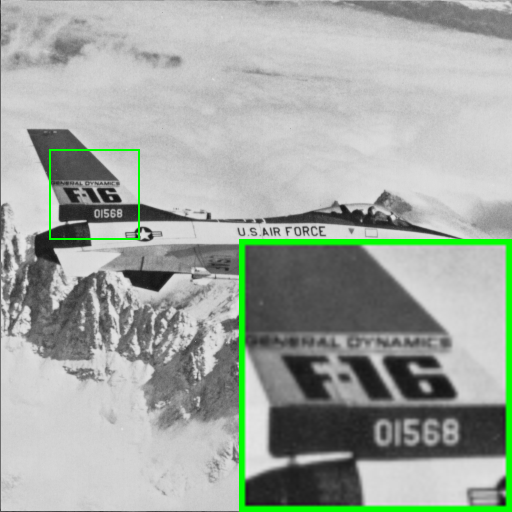
\includegraphics[width=1\textwidth]{images/pgpd/br_airplane.png}
	   \caption{Ground Truth}
    \end{subfigure}
    \hfill
    \begin{subfigure}[t]{0.24\textwidth}
        \centering
        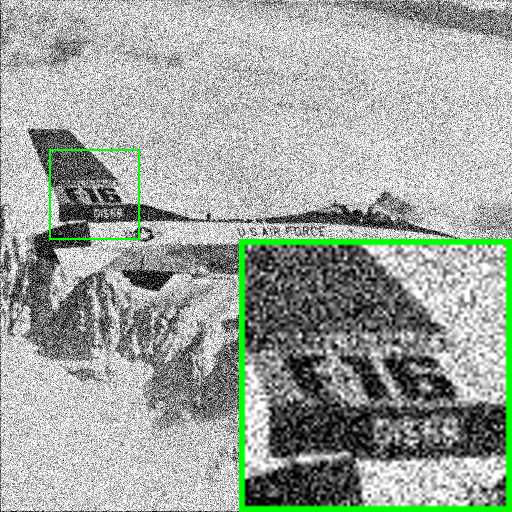
\includegraphics[width=1\textwidth]{images/pgpd/br_airplane_50.png}
		\caption{Noisy: 14.16}
    \end{subfigure}
    \hfill
    \begin{subfigure}[t]{0.24\textwidth}
        \centering
        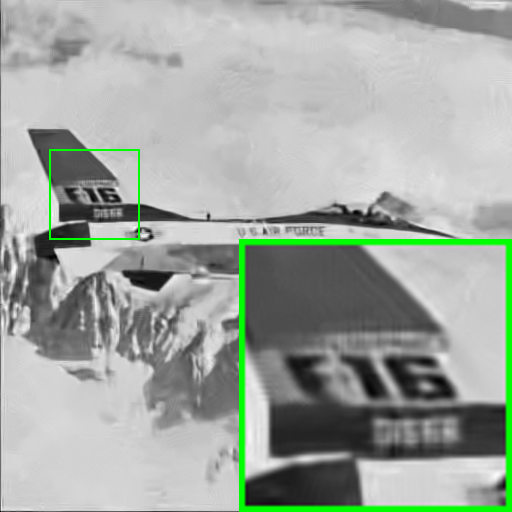
\includegraphics[width=1\textwidth]{images/pgpd/br_BM3D_50_airplane.png}
		\caption{BM3D: 28.24}
    \end{subfigure}
    \hfill
    \begin{subfigure}[t]{0.24\textwidth}
        \centering
        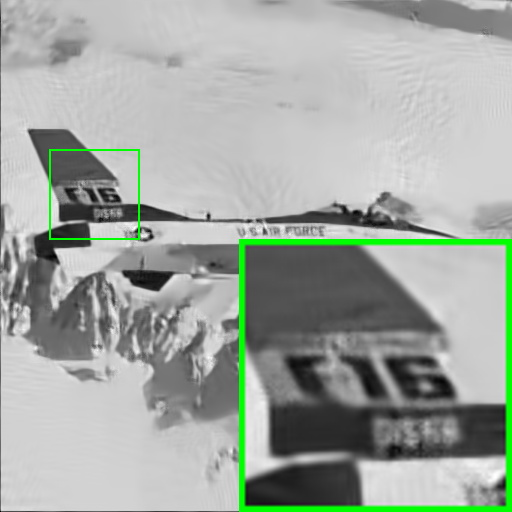
\includegraphics[width=1\textwidth]{images/pgpd/br_LSSC_50_airplane.png}
		\caption{LSSC: 28.15}
    \end{subfigure}
    \hfill
    \begin{subfigure}[t]{0.24\textwidth}
        \centering
        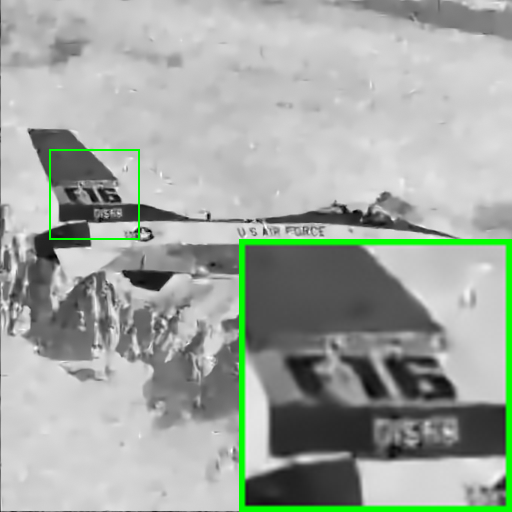
\includegraphics[width=1\textwidth]{images/pgpd/br_EPLL_50_airplane.png}
		\caption{EPLL: 28.19}
    \end{subfigure}
    \hfill
    \begin{subfigure}[t]{0.24\textwidth}
        \centering
        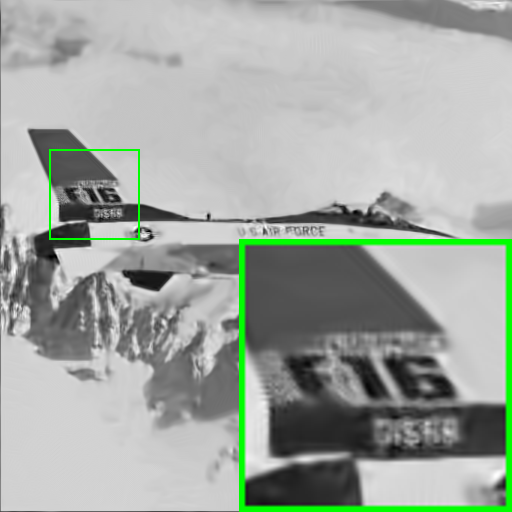
\includegraphics[width=1\textwidth]{images/pgpd/br_NCSR_50_airplane.png}
		\caption{NCSR: 28.18}
    \end{subfigure}
    \hfill
    \begin{subfigure}[t]{0.24\textwidth}
        \centering
        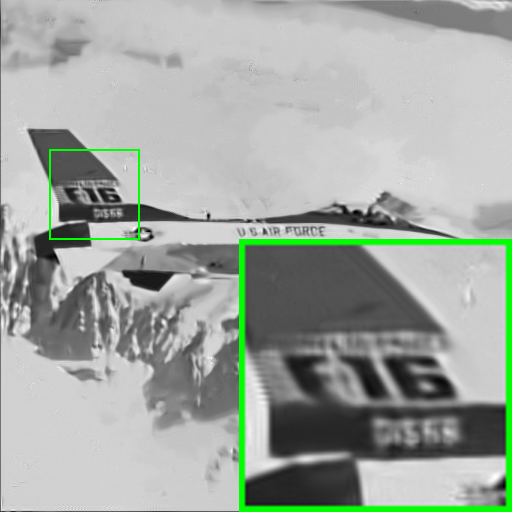
\includegraphics[width=1\textwidth]{images/pgpd/br_WNNM_50_airplane.png}
		\caption{WNNM: 28.55}
    \end{subfigure}
    \hfill
    \begin{subfigure}[t]{0.24\textwidth}
        \centering
        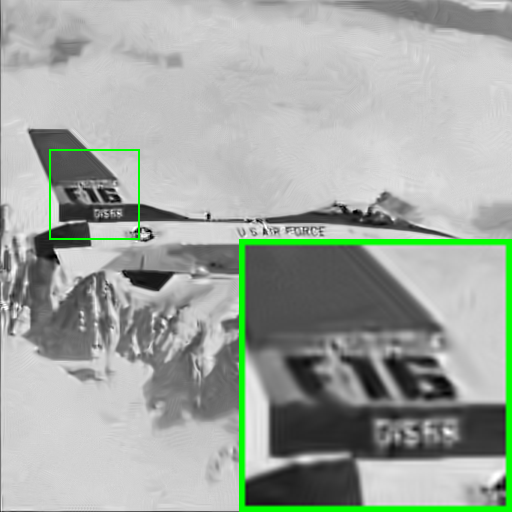
\includegraphics[width=1\textwidth]{images/pgpd/br_our_50_airplane.png}
		\caption{PGPD: 28.38}
    \end{subfigure}
    \caption{Denoised images and PSNR (dB) results of \textsl{Airplane} by different methods (the standard deviation of noise is $\sigma=50$).}
    \label{fig6}
\end{figure}



\begin{figure}
    \centering
    \begin{subfigure}[t]{0.24\textwidth}
        \centering
        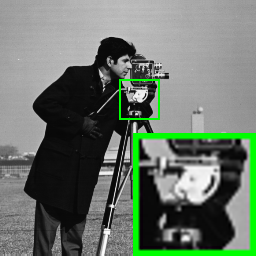
\includegraphics[width=1\textwidth]{images/pgpd/br_cameraman.png}
	   \caption{Ground Truth}
    \end{subfigure}
    \hfill
    \begin{subfigure}[t]{0.24\textwidth}
        \centering
        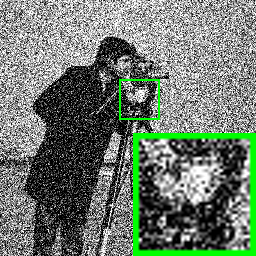
\includegraphics[width=1\textwidth]{images/pgpd/br_cameraman_75.png}
		\caption{Noisy: 10.60}
    \end{subfigure}
    \hfill
    \begin{subfigure}[t]{0.24\textwidth}
        \centering
        \includegraphics[width=1\textwidth]{images/pgpd/br_BM3D_75_cameraman.png}
		\caption{BM3D: 24.33}
    \end{subfigure}
    \hfill
    \begin{subfigure}[t]{0.24\textwidth}
        \centering
        \includegraphics[width=1\textwidth]{images/pgpd/br_LSSC_75_cameraman.png}
		\caption{LSSC: 24.41}
    \end{subfigure}
    \hfill
    \begin{subfigure}[t]{0.24\textwidth}
        \centering
        \includegraphics[width=1\textwidth]{images/pgpd/br_EPLL_75_cameraman.png}
		\caption{EPLL: 24.29}
    \end{subfigure}
    \hfill
    \begin{subfigure}[t]{0.24\textwidth}
        \centering
        \includegraphics[width=1\textwidth]{images/pgpd/br_NCSR_75_cameraman.png}
		\caption{NCSR: 24.22}
    \end{subfigure}
    \hfill
    \begin{subfigure}[t]{0.24\textwidth}
        \centering
        \includegraphics[width=1\textwidth]{images/pgpd/br_WNNM_75_cameraman.png}
		\caption{WNNM: 24.55}
    \end{subfigure}
    \hfill
    \begin{subfigure}[t]{0.24\textwidth}
        \centering
        \includegraphics[width=1\textwidth]{images/pgpd/br_our_75_cameraman.png}
		\caption{PGPD: 24.64}
    \end{subfigure}
    \caption{Denoised images and PSNR (dB) results of \textsl{Cameraman} by different methods (the standard deviation of noise is $\sigma=75$).}
    \label{fig7}
\end{figure}



\section{Conclusion}
How to learn explicit models of nonlocal self-similarity (NSS) prior for image restoration is an open problem, and we made a good attempt on this by lifting the patch based image modeling to patch group (PG) based image modeling. A PG is a group of similar patches in an image region. After group mean subtraction, a PG can naturally represent the NSS variations of natural images. A PG based Gaussian Mixture Model (PG-GMM) learning algorithm was developed to learned the NSS prior from natural images, and an associated weighted sparse coding algorithm was developed for high performance image denoising. The so-called \textsl{PG Prior based Denoising} (PGPD) algorithm not only achieves highly competitive PSNR results with state-of-the-art denoising methods, but also is highly efficient and preserves better the image edges and textures. The proposed method can be extended to other image processing tasks such as deblurring and super-resolution.
